%%%%%%%%%%%%%%%%%%%%%%%%%%%%%%%%%%%%%%%%%
% Short Sectioned Assignment
% LaTeX Template
% Version 1.0 (5/5/12)
%
% This template has been downloaded from:
% http://www.LaTeXTemplates.com
%
% Original author:
% Frits Wenneker (http://www.howtotex.com)
%
% License:
% CC BY-NC-SA 3.0 (http://creativecommons.org/licenses/by-nc-sa/3.0/)
%
%%%%%%%%%%%%%%%%%%%%%%%%%%%%%%%%%%%%%%%%%

%----------------------------------------------------------------------------------------
%	PACKAGES AND OTHER DOCUMENT CONFIGURATIONS
%----------------------------------------------------------------------------------------

\documentclass[paper=a4, fontsize=12pt]{scrartcl} % A4 paper and 11pt font size

\usepackage[T1]{fontenc} % Use 8-bit encoding that has 256 glyphs
\usepackage{fourier} % Use the Adobe Utopia font for the document - comment this line to return to the LaTeX default
\usepackage[english]{babel} % English language/hyphenation
\usepackage{amsmath,amsfonts,amsthm} % Math packages

\usepackage{sectsty} % Allows customizing section commands
\allsectionsfont{\centering \normalfont\scshape} % Make all sections centered, the default font and small caps

\usepackage{graphicx}

\usepackage[a4paper,lmargin=2.5 cm,rmargin=2 cm,tmargin=2 cm,bmargin=2 cm]{geometry}

\usepackage{fancyhdr} % Custom headers and footers
\pagestyle{fancyplain} % Makes all pages in the document conform to the custom headers and footers
\fancyhead{} % No page header - if you want one, create it in the same way as the footers below
\fancyfoot[L]{} % Empty left footer
\fancyfoot[C]{} % Empty center footer
\fancyfoot[C]{\thepage} % Page numbering for right footer
\renewcommand{\headrulewidth}{0pt} % Remove header underlines
\renewcommand{\footrulewidth}{0pt} % Remove footer underlines
\setlength{\headheight}{13.6pt} % Customize the height of the header

\usepackage{chngcntr}
%\numberwithin{equation}{section} % Number equations within sections (i.e. 1.1, 1.2, 2.1, 2.2 instead of 1, 2, 3, 4)
%\numberwithin{figure}{section} % Number figures within sections (i.e. 1.1, 1.2, 2.1, 2.2 instead of 1, 2, 3, 4)
%\counterwithout{figure}{section}
%\numberwithin{table}{section} % Number tables within sections (i.e. 1.1, 1.2, 2.1, 2.2 instead of 1, 2, 3, 4)

\setlength\parindent{0pt} % Removes all indentation from paragraphs - comment this line for an assignment with lots of text

\usepackage{amsmath}
\usepackage{float} % To firce the location of figure
\usepackage{subfigure} %For side-by-side figures
\usepackage{lettrine}
%\usepackage{lipsum}
\usepackage{epstopdf} %To read *.eps Files
\usepackage{listings} % To include source codes in LATEX document
\usepackage{mathrsfs} % To include script fonts. use \mathscr{}
\usepackage{courier} % To write in courier fornt
\usepackage{mathtools} % For mat symbols
\usepackage{xfrac} % For \sfrac{}{}
\usepackage{pdfpages} % To insert Pdf files
%----------------------------------------------------------------------------------------
%	TITLE SECTION
%----------------------------------------------------------------------------------------

\newcommand{\horrule}[1]{\rule{\linewidth}{#1}} % Create horizontal rule command with 1 argument of height

\title{	
\normalfont \normalsize 
\textsc{Wright State University\\ Department of Mechanical and Materials Engineering} \\ [25pt] % Your university, school and/or department name(s)
\horrule{0.5pt} \\[0.4cm] % Thin top horizontal rule
\large ME7690 - Vibration Testing and Machine Health Monitoring \\ % The assignment title
\huge System Identification using Frequency Domain Modal Analysis\\
\horrule{2pt} \\[0.5cm] % Thick bottom horizontal rule
}

\author{Koorosh Gobal} % Your name

\date{\normalsize\today} % Today's date or a custom date

\begin{document}

\maketitle % Print the title

%----------------------------------------------------------------------------------------
%	SECTION 1
%----------------------------------------------------------------------------------------
\section*{Problem Description}
Experimental modal analysis has become a commonly-used technique for studying the dynamical behavior of mechanical and civil structures, such as cars, aircrafts, bridges and industrial machinery. During a modal test, both the applied forces and vibration responses of the structure are measured when excited in one or more locations. Based on this data, a modal model of the structure, that essentially contains the same information as the original vibration data, is derived by means of system identification. The identification techniques are categorized based on number of degrees of freedom of the system and number of inputs/outputs.
%----------------------------------------------------------------------------------------
%	SECTION 1
%----------------------------------------------------------------------------------------
\section*{Methodology}
\subsection*{Single Degree of Freedom Curve Fitting with Residual}
\lq\lq Single Degree of Freedom Curve Fitting with Residual\rq\rq\ is one of the methods that is used when several natural frequencies occur in the FRF data. Each of these frequencies contribute over the entire frequency range. Therefore, when fitting a curve to a single peak, the effect of other natural frequencies should be accounted in the procedure. Therefore, the residuals are introduced to compensate the effect of other natural frequencies when fitting only one peak. This is shown in Equation \eqref{eq:SDOFwR}. It should be noted that $R_I$ and $R_K$ represent residual contributions from the lower and high frequency modes and does not have any physical meaning.
%
\begin{gather}\label{eq:SDOFwR}
	H(j\omega) = R_I + \frac{1}{-\omega^2 m + j\omega c + k} + R_K
\end{gather}
%
With some manipulation, above can be written as a ration of two polynomials as
%
\begin{gather}
	H(j\omega) = \frac{\alpha_4 (j\omega)^4 + \alpha_3 (j\omega)^3 + \alpha_2 (j
	\omega)^2 + \alpha_1 (j\omega) + \alpha_0}{\beta_4 (j\omega)^4 + \beta_3 (j
	\omega)^3 + \beta_2 (j\omega)^2}
\end{gather}
%
This can be written in for all the frequency range around one of the peaks in the matrix form as
%
\begin{gather}\label{SDOFwR_matix}
\begin{bmatrix}
	(j\omega_1)^2 H(j\omega_1) & (j\omega_1)^3 H(j\omega_1) & -(j\omega_1)^0 & 
	\dots & -(j\omega_1)^4 \\
	(j\omega_2)^2 H(j\omega_2) & (j\omega_2)^3 H(j\omega_2) & -(j\omega_2)^0 & 
	\dots & -(j\omega_2)^4 \\
	\vdots & \vdots & \vdots & \ddots & \vdots \\
	(j\omega_{n_s})^2 H(j\omega_{n_s}) & (j\omega_{n_s})^3 H(j\omega_{n_s}) & -(j
	\omega_{n_s})^0 & \dots & -(j\omega_{n_s})^4 \\
\end{bmatrix}
\begin{bmatrix}
	\beta_2 \\
	\beta_1 \\
	\alpha_0 \\
	\alpha_1 \\
	\alpha_2 \\
	\alpha_3 \\
	\alpha_4
\end{bmatrix}
=
\begin{bmatrix}
	j\omega_1)^4 H(j\omega_1) \\
	j\omega_2)^4 H(j\omega_2) \\
	\vdots \\
	j\omega_{n_s})^4 H(j\omega_{n_s})
\end{bmatrix}
\end{gather}
%
After solving Equation \eqref{SDOFwR_matix}, the two nonzero roots of the polynomial $\lambda^4 + \beta_3 \lambda^3 + \beta_2 \lambda^2 + 0 + 0 = 0$ yield the poles of the system. The natural frequency and damping coefficient can be calculated using the following equations.
%
\begin{subequations}
\begin{align}
	\omega_n = ||\lambda|| \\
	\zeta = -\frac{\text{real}(\lambda)}{||\lambda||}
\end{align}
\end{subequations}
%
Furthermore, this can be followed by a subsequent curve fit to obtain the residue as follows.
%
\begin{gather}
\begin{bmatrix}
	H(j\omega_1) \\
	H(j\omega_2) \\
	\vdots \\
	H(j\omega_{n_s})
\end{bmatrix}
=
\begin{bmatrix}
	-\frac{1}{\omega_1^2} & 1 & \frac{1}{j\omega_1 - \lambda_1} & \frac{1}{j
	\omega_1 - \bar{\lambda}_1} \\
	-\frac{1}{\omega_2^2} & 1 & \frac{1}{j\omega_2 - \lambda_2} & \frac{1}{j
	\omega_2 - \bar{\lambda}_2} \\
	\vdots & \vdots & \vdots & \vdots \\
	-\frac{1}{\omega_{n_s}^2} & 1 & \frac{1}{j\omega_{n_s} - \lambda_{n_s}} & 
	\frac{1}{j\omega_{n_s} - \bar{\lambda}_{n_s}}
\end{bmatrix}
\begin{bmatrix}
	\frac{1}{m_r} \\
	\frac{1}{k_r} \\
	b \\
	\bar{b}
\end{bmatrix}
\end{gather}
%
The value for the residues can be used to qualify the fitted curve.
% --------------------------------------------------------------------------------
\subsection*{MDOF Curve Fitting - Single Input Collocated with Sensor}
It is possible to curve fit a large number of FRFs simultaneously to approximate different properties of the system. The \lq\lq MDOF Curve Fitting\rq\rq\ is used when the system is defined to have a single input at a location where the is also a sensor. This method will work provided that the number of modes appearing in the FRFs is equal to the number of sensors.\\

For the range of $n_s$ frequencies in the domain, the second order equation of motion can be written in the matrix form as
%
\begin{gather}\label{eq:MDOF}
\begin{bmatrix}
	-\omega_1^2 \mathbf{H}(j\omega_1)^T & j\omega_1 \mathbf{H}(j\omega_1)^T & 
	\mathbf{H}(j\omega_1)^T \\
	-\omega_2^2 \mathbf{H}(j\omega_2)^T & j\omega_2 \mathbf{H}(j\omega_2)^T & 
	\mathbf{H}(j\omega_2)^T \\
	\vdots & \vdots & \vdots \\
	-\omega_{n_s}^2 \mathbf{H}(j\omega_{n_s})^T & j\omega_{n_s} \mathbf{H}(j
	\omega_{n_s})^T & \mathbf{H}(j\omega_{n_s})^T \\
\end{bmatrix}
\begin{bmatrix}
	\mathbf{M} \\
	\mathbf{C} \\
	\mathbf{K}
\end{bmatrix}
=
\begin{bmatrix}
	\tilde{\mathbf{B}}^T \\
	\tilde{\mathbf{B}}^T \\
	\vdots \\
	\tilde{\mathbf{B}}^T
\end{bmatrix}
\end{gather}
%
it should be noted that the $\mathbf{H}(j\omega)$ is the full FRF matrix as shown in the following equation. Where \lq\lq$o$\rq\rq , represents the inputs and \lq\lq$p$\rq\rq\ represents the output.
%
\begin{gather}
\mathbf{H}(\omega) =
\begin{bmatrix}
	H_{1,1}(\omega) & H_{1,2}(\omega) & \cdots & H_{1,o}(\omega) \\
	H_{2,1}(\omega) & H_{2,2}(\omega) &  & \vdots \\
	\vdots &  & \ddots &  \\
	H_{p,1}(\omega)	& \cdots &  & H_{p,o}(\omega)
\end{bmatrix}
\end{gather}
%
%----------------------------------------------------------------------------------------
%	SECTION 1
%----------------------------------------------------------------------------------------
\section*{Experimental Setup}
In this lab, we derive the system properties of the cruise missile wing that is available in the vibrations lab. Three accelerometers are placed on the test article (wing) and the model is excited using the hammer. The excitation locations are collocated with sensors so we can use MDOF method afterwards. The test setup is shown in Figure ~\ref{fig:test_setup} where accelerometers are shown using white arrow. In this lab, we have used \lq\lq Single Degree of Freedom Curve Fitting with Residual\rq\rq\ and \lq\lq MDOF Curve fitting\rq\rq\ to identify the system properties.
%
\begin{figure}[H]
	\centering
	\includegraphics[height = 8.5cm]{test_setup.jpg}
	\caption{The experimental setup.}
	\label{fig:test_setup}
\end{figure}
%
%----------------------------------------------------------------------------------------
%	SECTION 1
%----------------------------------------------------------------------------------------
\section*{Results and Discussion}
Data is collected by exciting the test article at the collocated locations with the accelerometers. For each excitation, 10 sets of realizations were gathered for post processing. This raw time domain data is then transferred to the frequency domain using Matlab's \texttt{fft} function. Based on the frequency domain data, the auto and spectral density functions are calculated for each realization. The auto and spectral density functions are averaged in the frequency domain and used to calculate two different frequency response functions as described in Equation \eqref{eq:H1H2}. The coherence is also calculate to quantify the quality of the FRF estimates. As shown in Figures ~\ref{fig:all_FRFs_1}, ~\ref{fig:all_FRFs_2} and ~\ref{fig:all_FRFs_3}, the coherence is around one in most of the frequency range. This represents a good quality FRF.
%
\begin{subequations}\label{eq:H1H2}
\begin{align}
H_1(j\omega) &= \frac{G_{fx}(j\omega)}{G_{ff}(j\omega)} \\
H_2(j\omega) &= \frac{G_{xx}(j\omega)}{G_{xf}(j\omega)}
\end{align}
\end{subequations}
%
%
\begin{figure}[H]
	\centering
	\subfigure[]
	{
		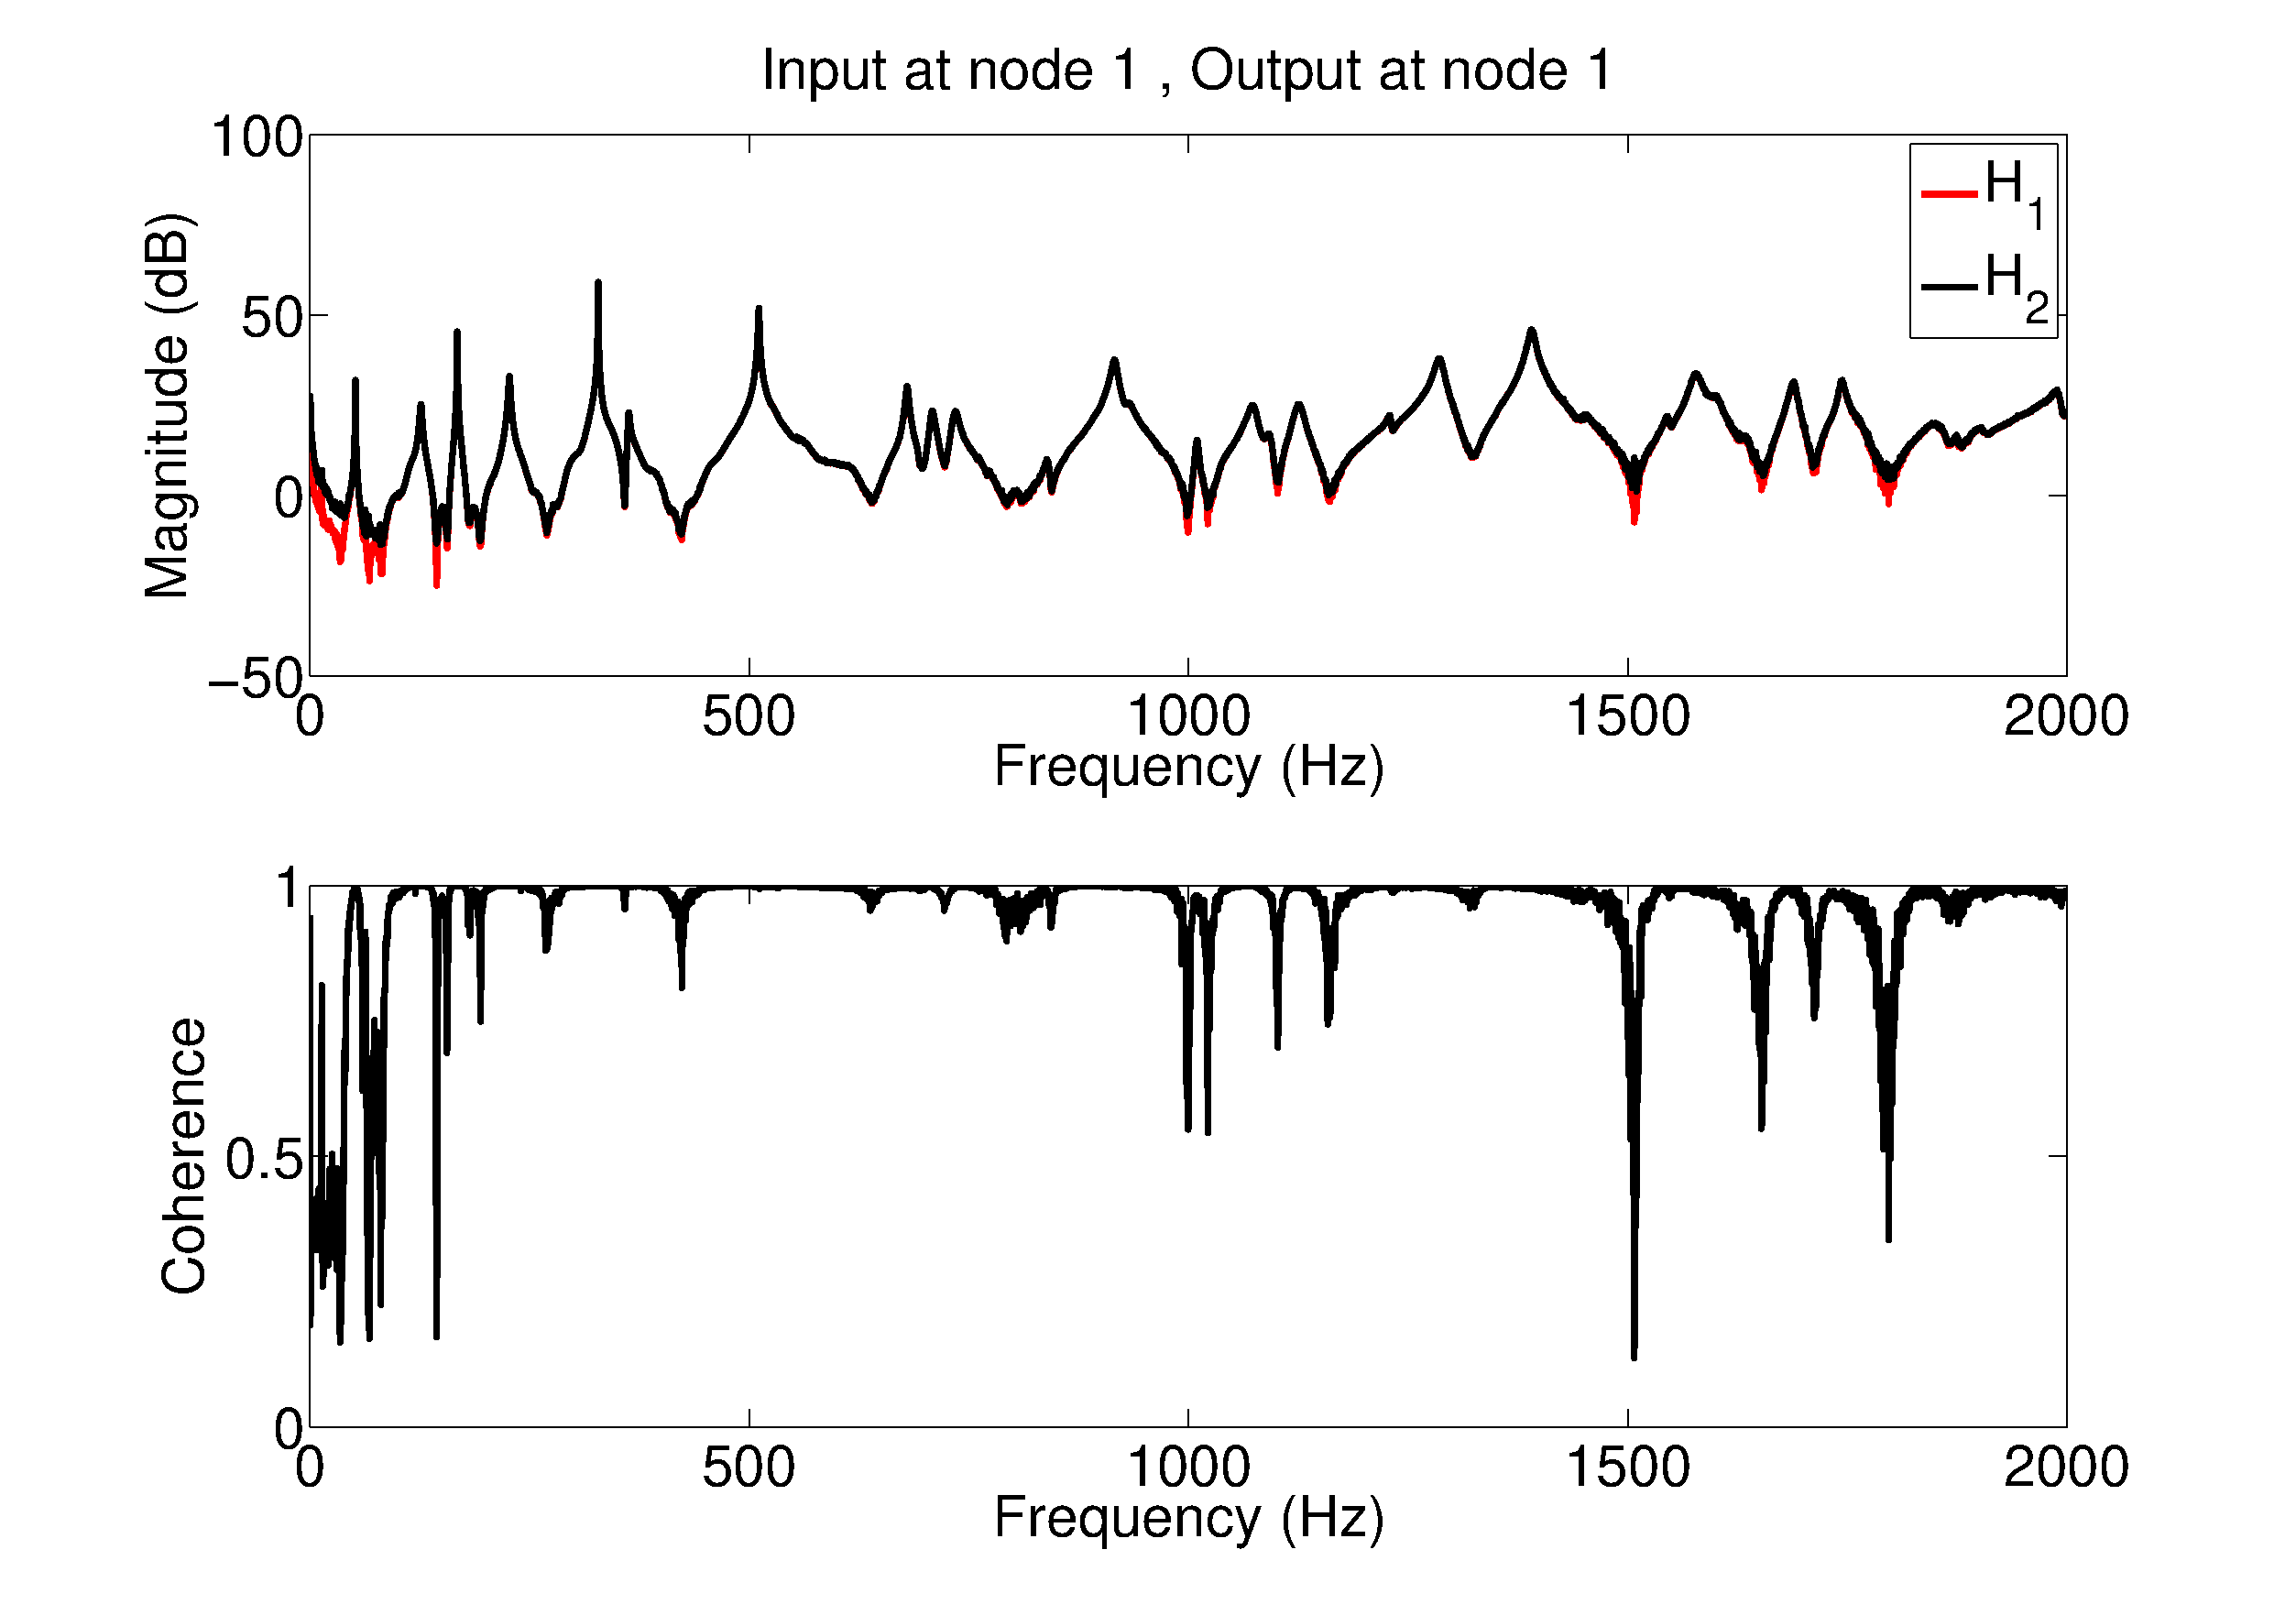
\includegraphics[height=4.75cm]{H11.eps}
	}
	\quad
	\subfigure[]
	{
		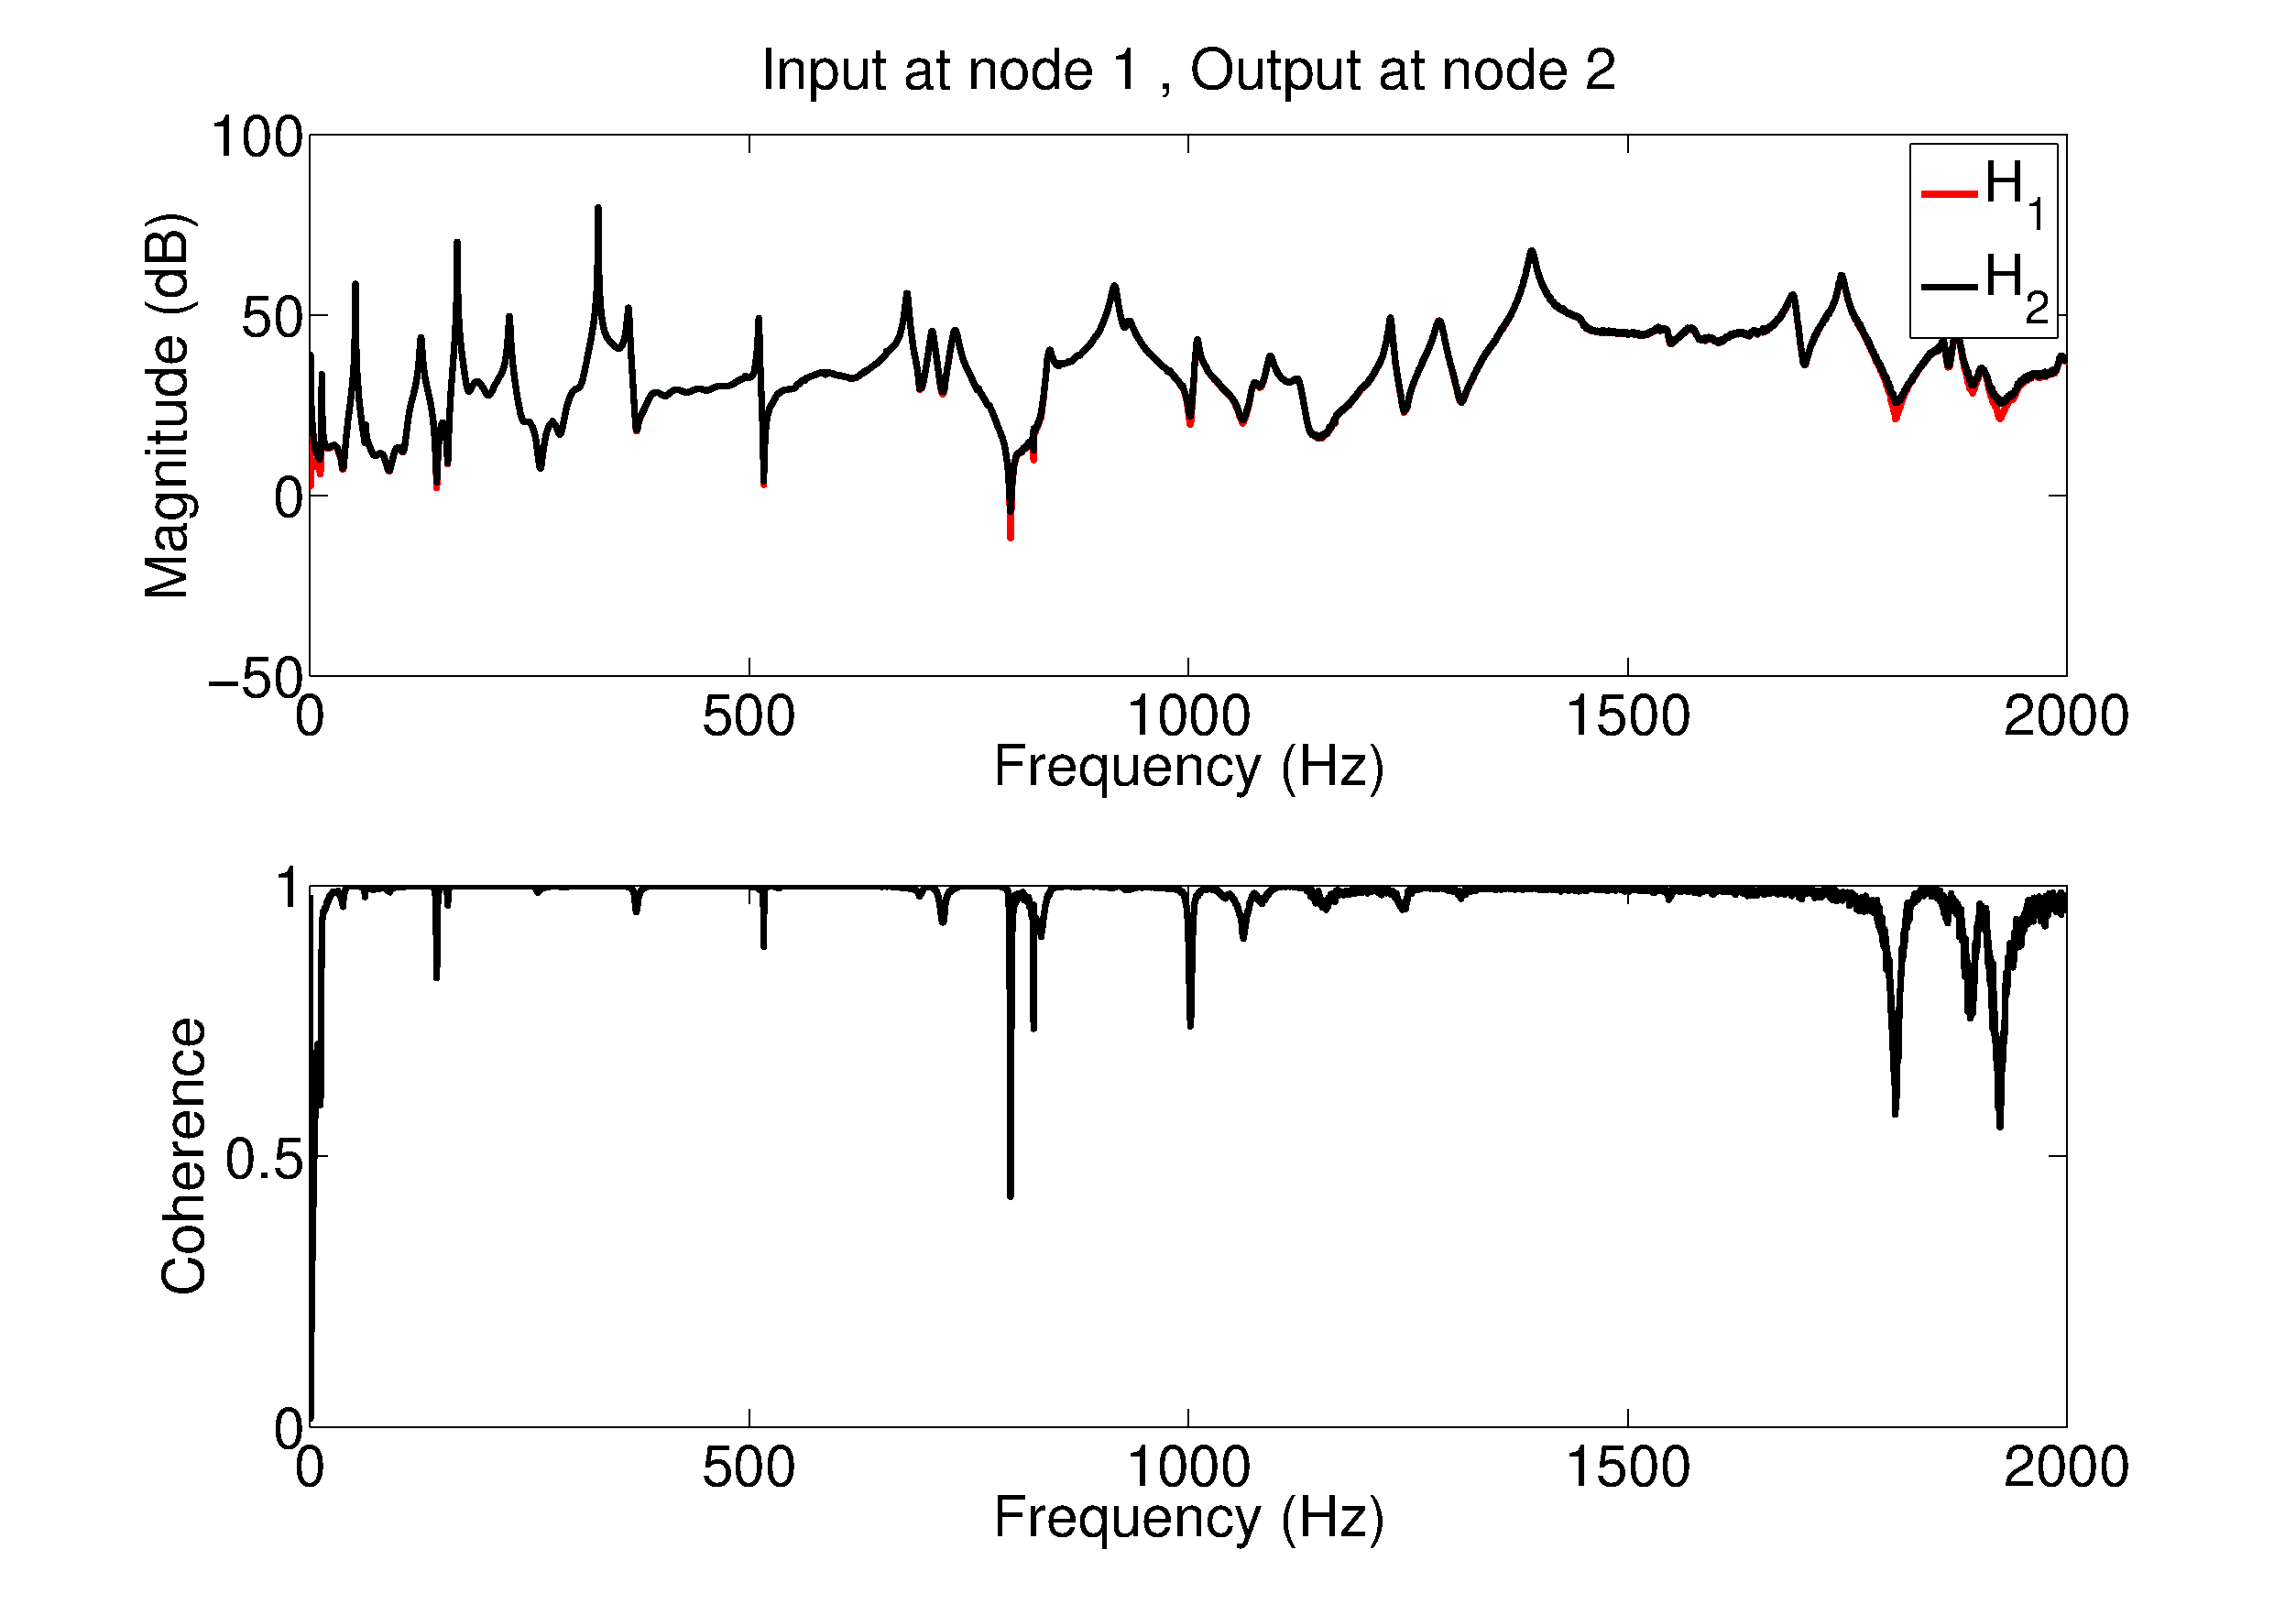
\includegraphics[height=4.75cm]{H21.eps}
	}
	\\
	\subfigure[]
	{
		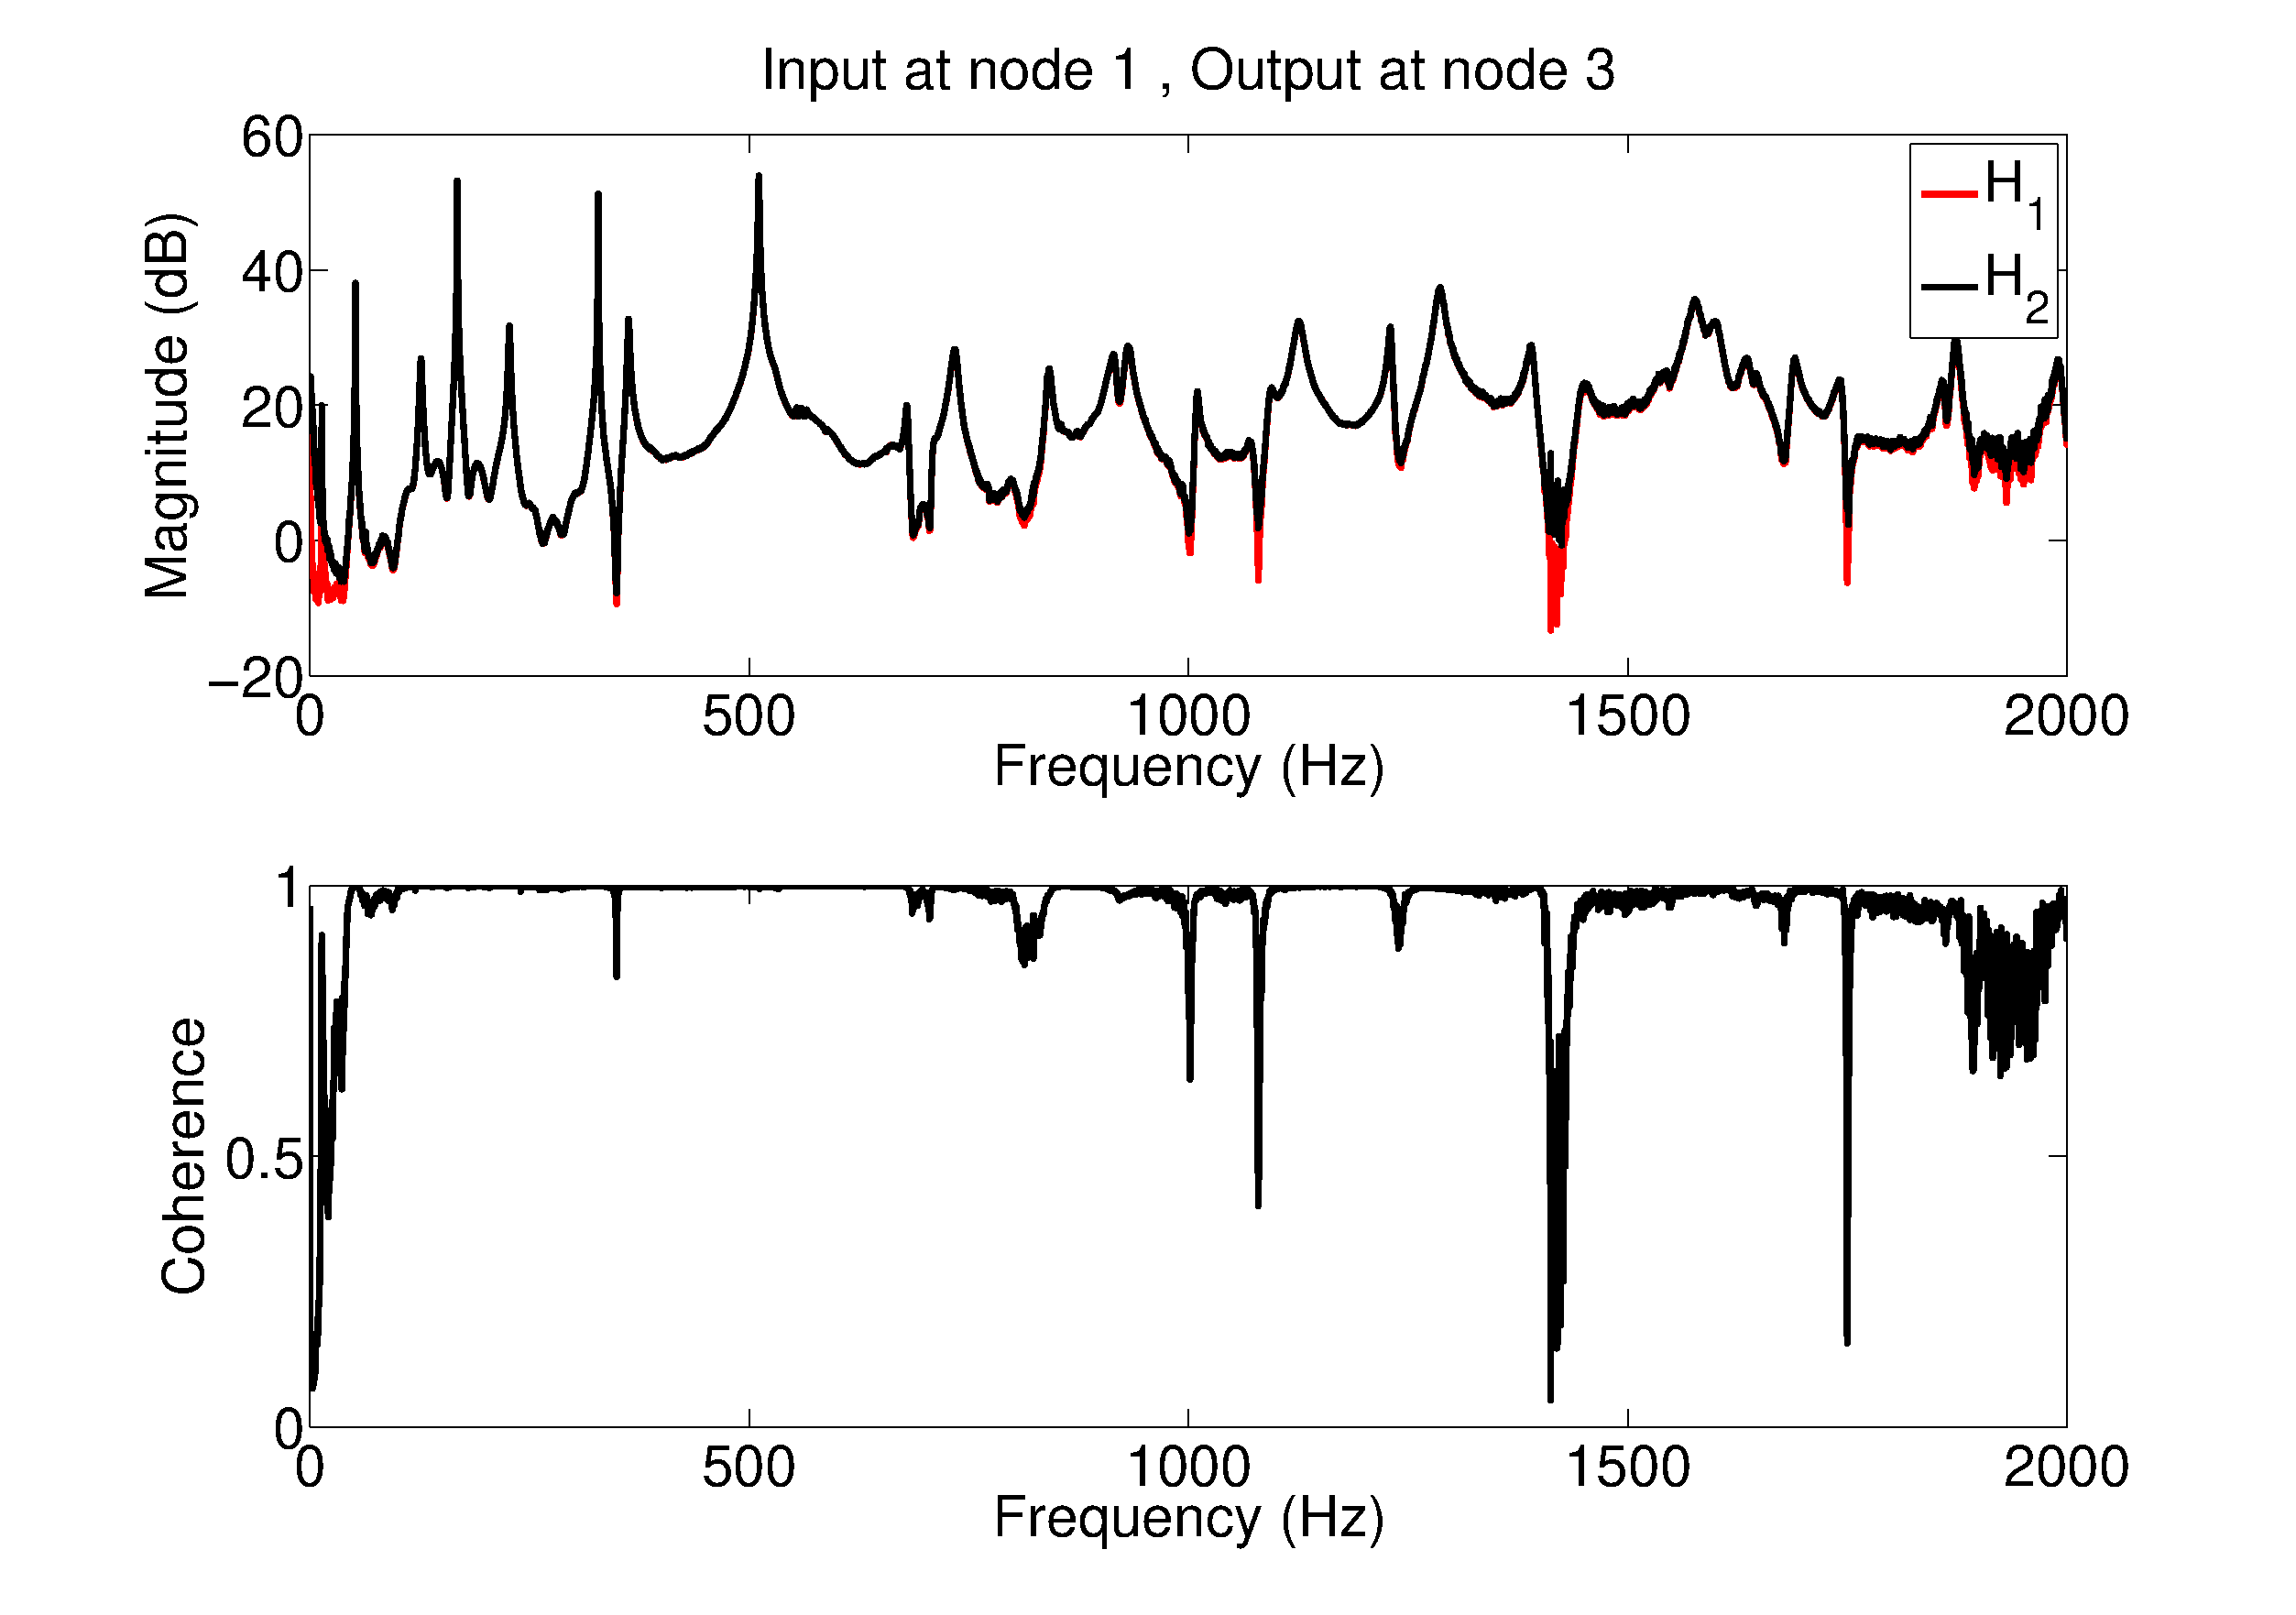
\includegraphics[height=4.75cm]{H31.eps}
	}
	\caption{Frequency response function for input at node 1.}
	\label{fig:all_FRFs_1}
\end{figure}
%
%
\begin{figure}[H]
	\centering
	\subfigure[]
	{
		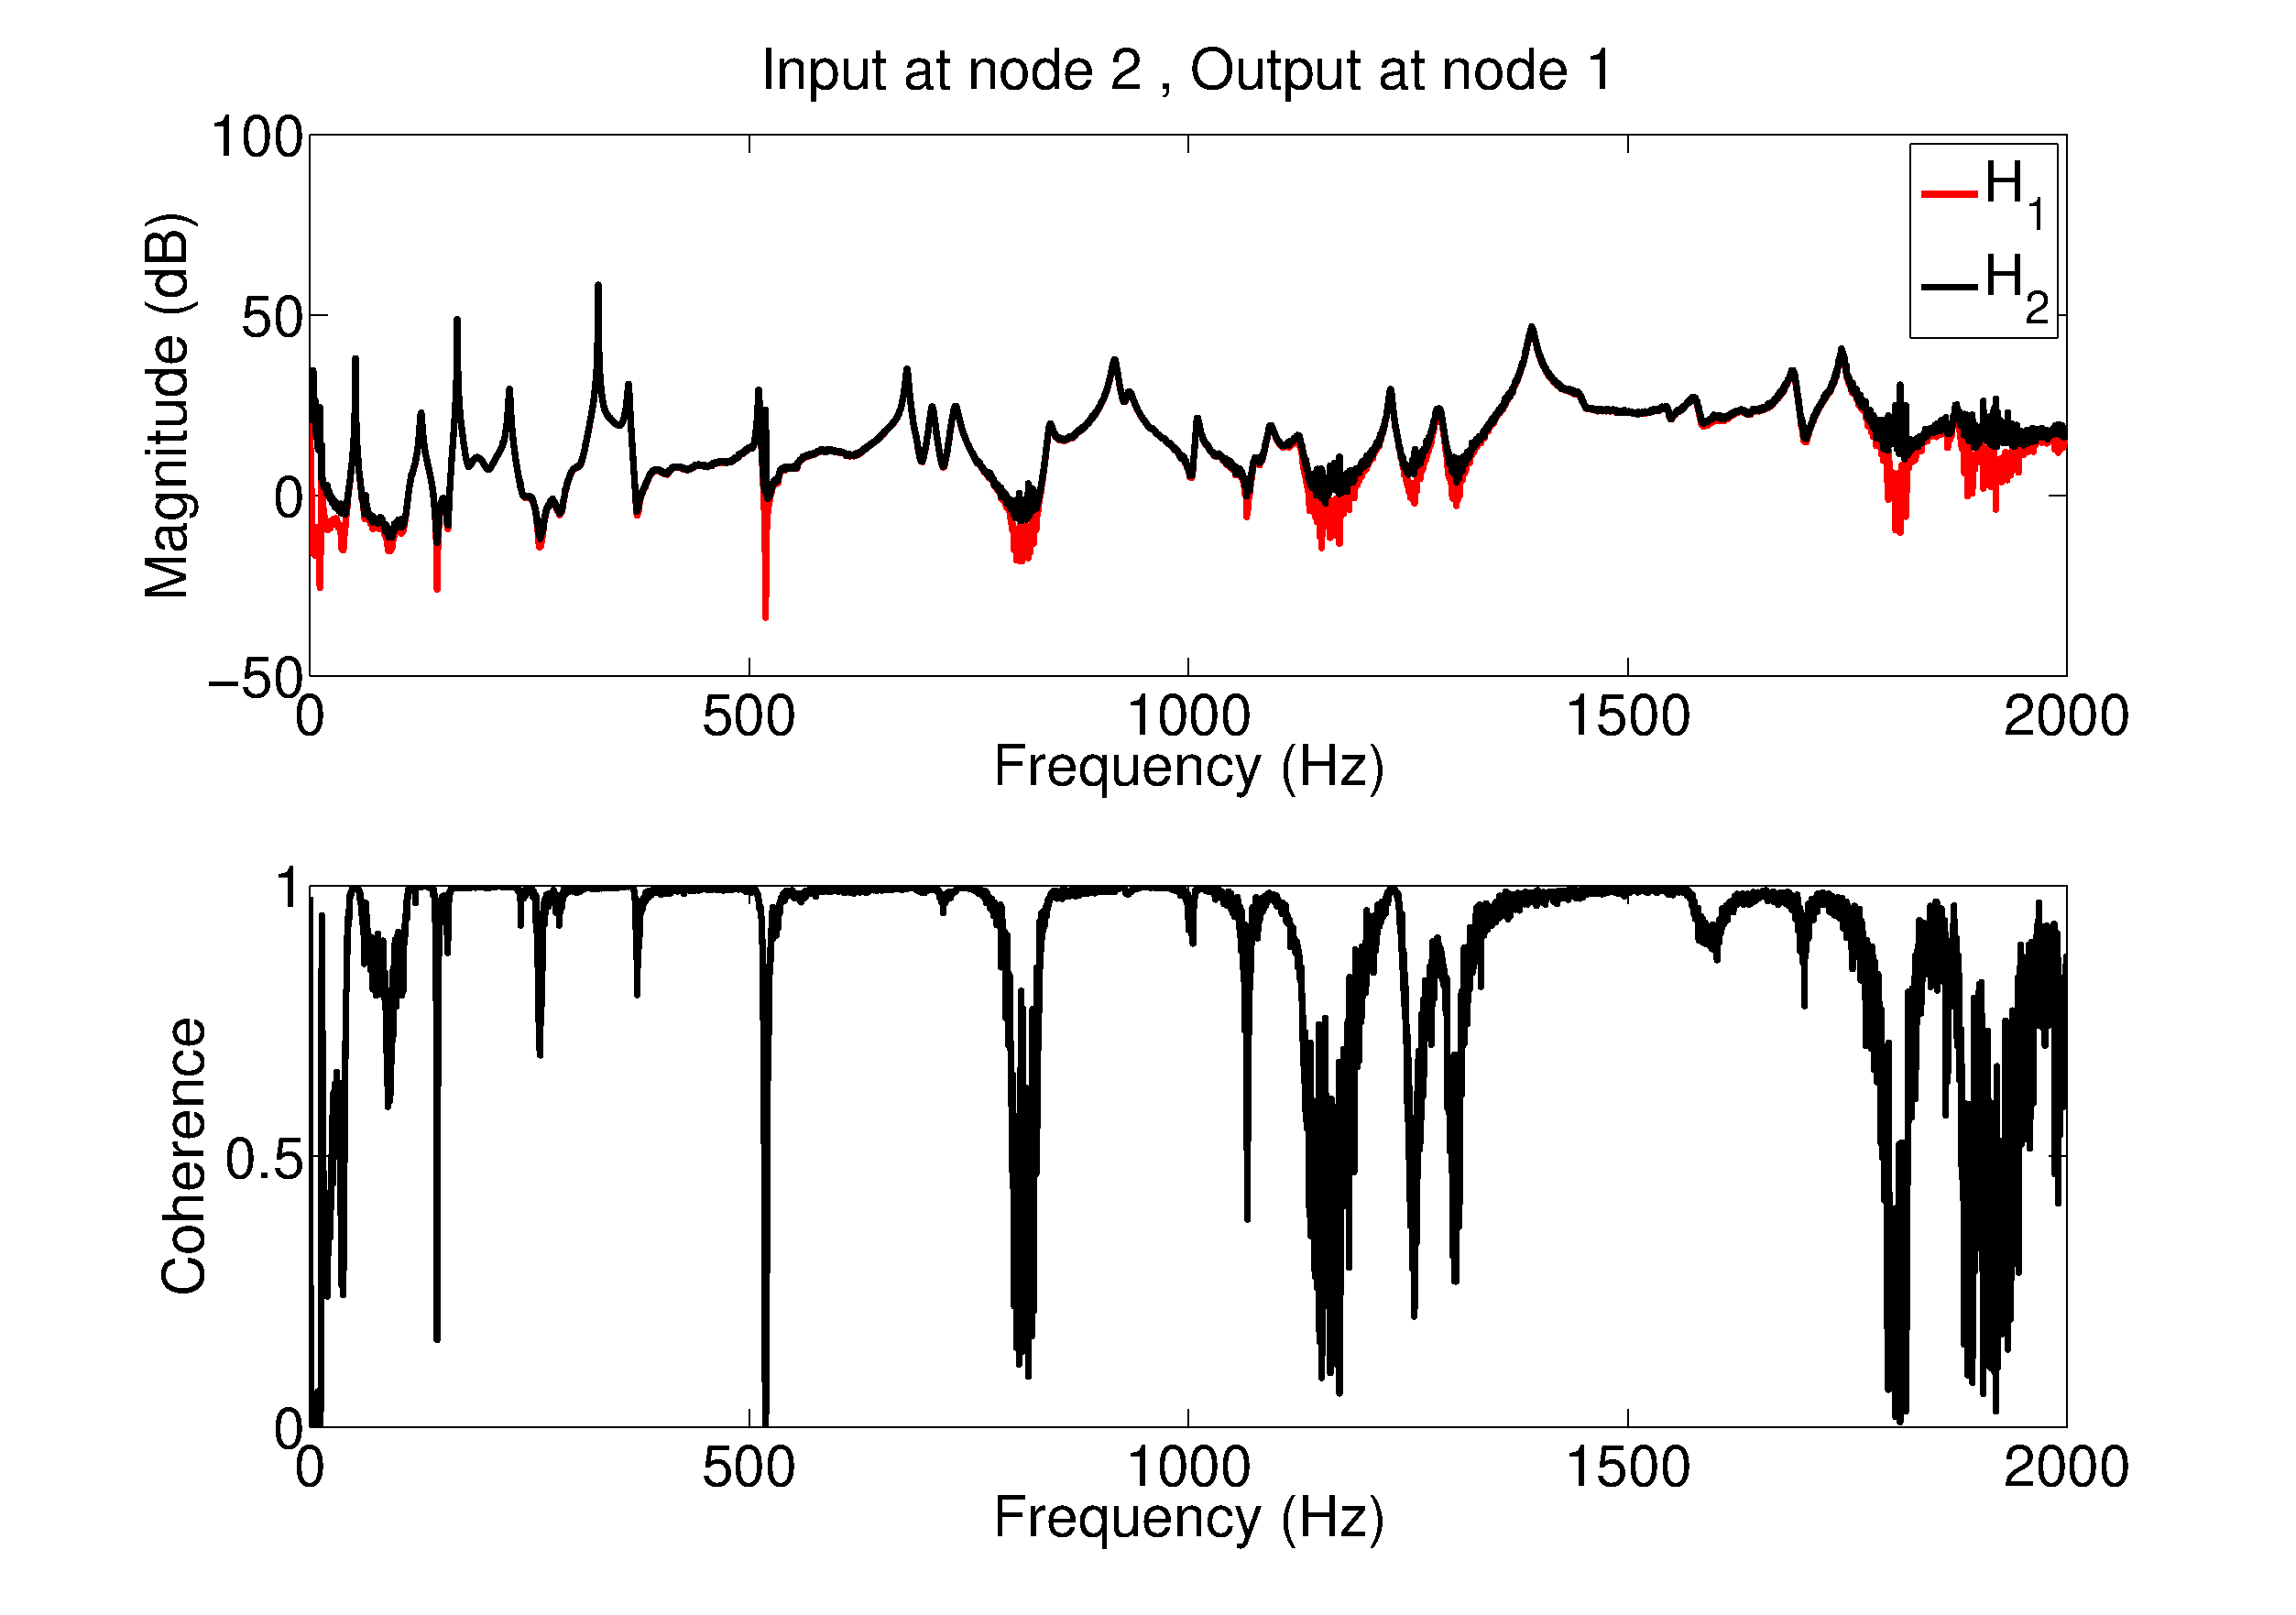
\includegraphics[height=4.75cm]{H12.eps}
	}
	\quad
	\subfigure[]
	{
		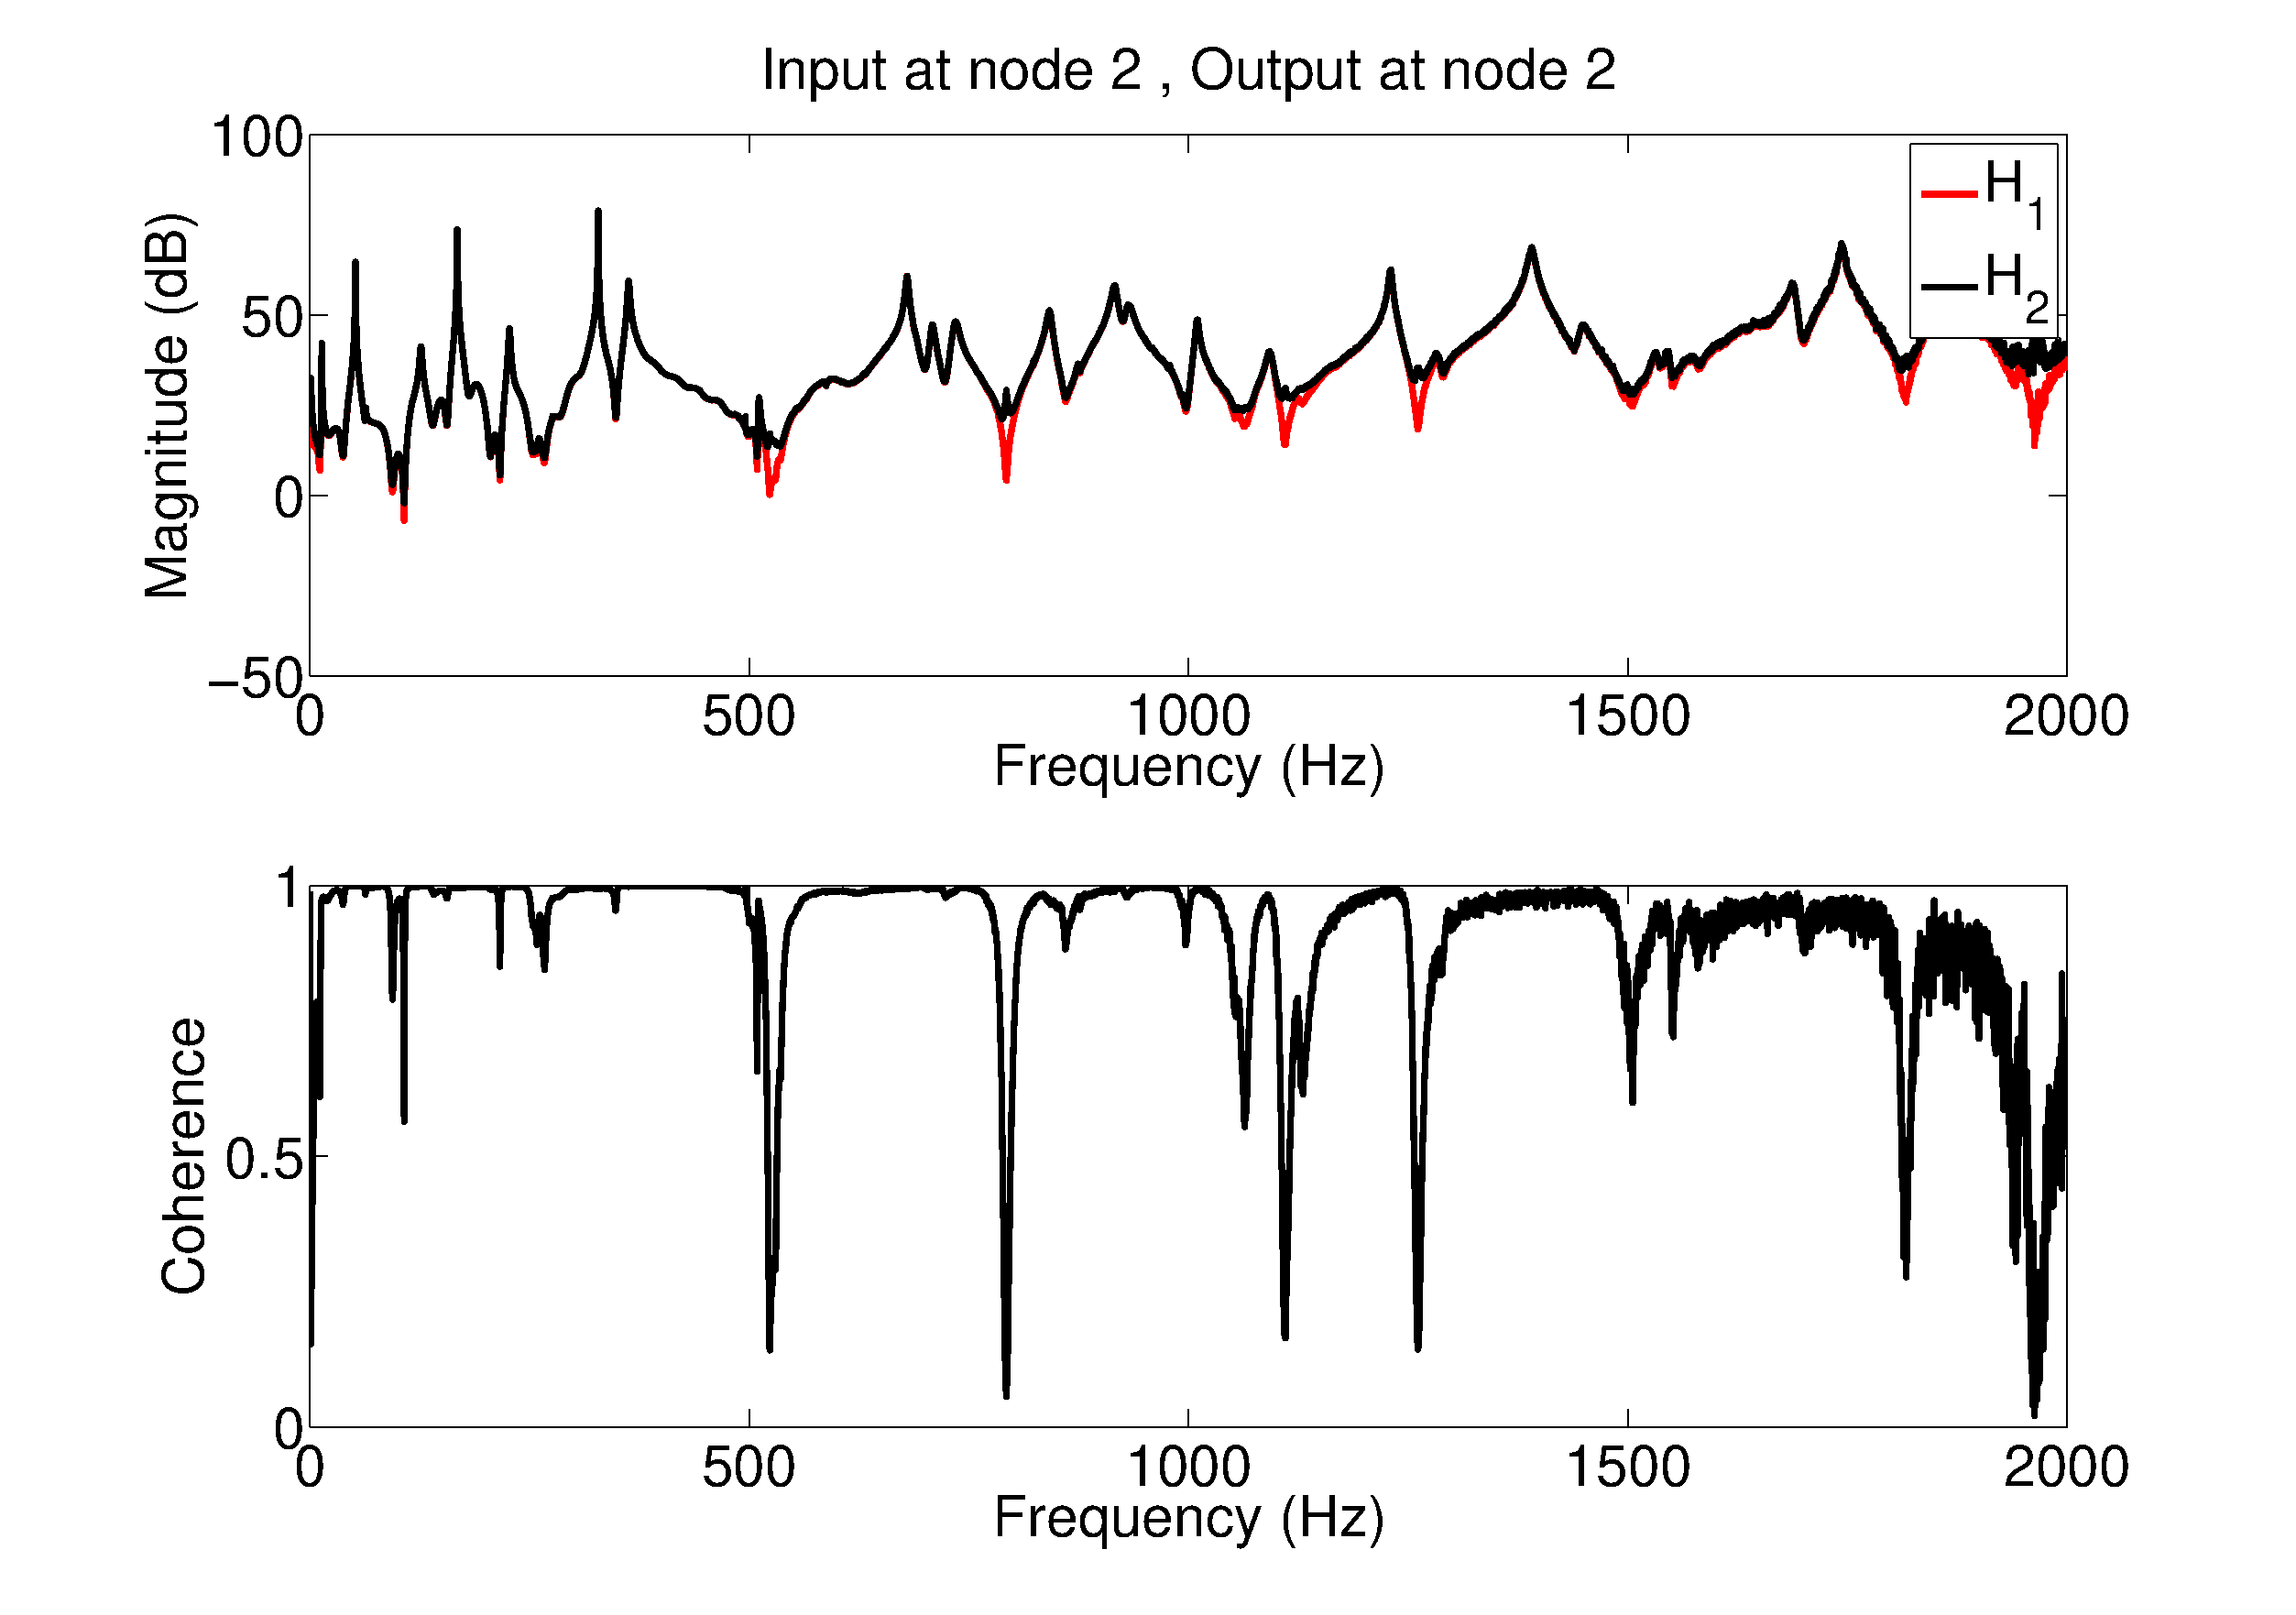
\includegraphics[height=4.75cm]{H22.eps}
	}
	\\
	\subfigure[]
	{
		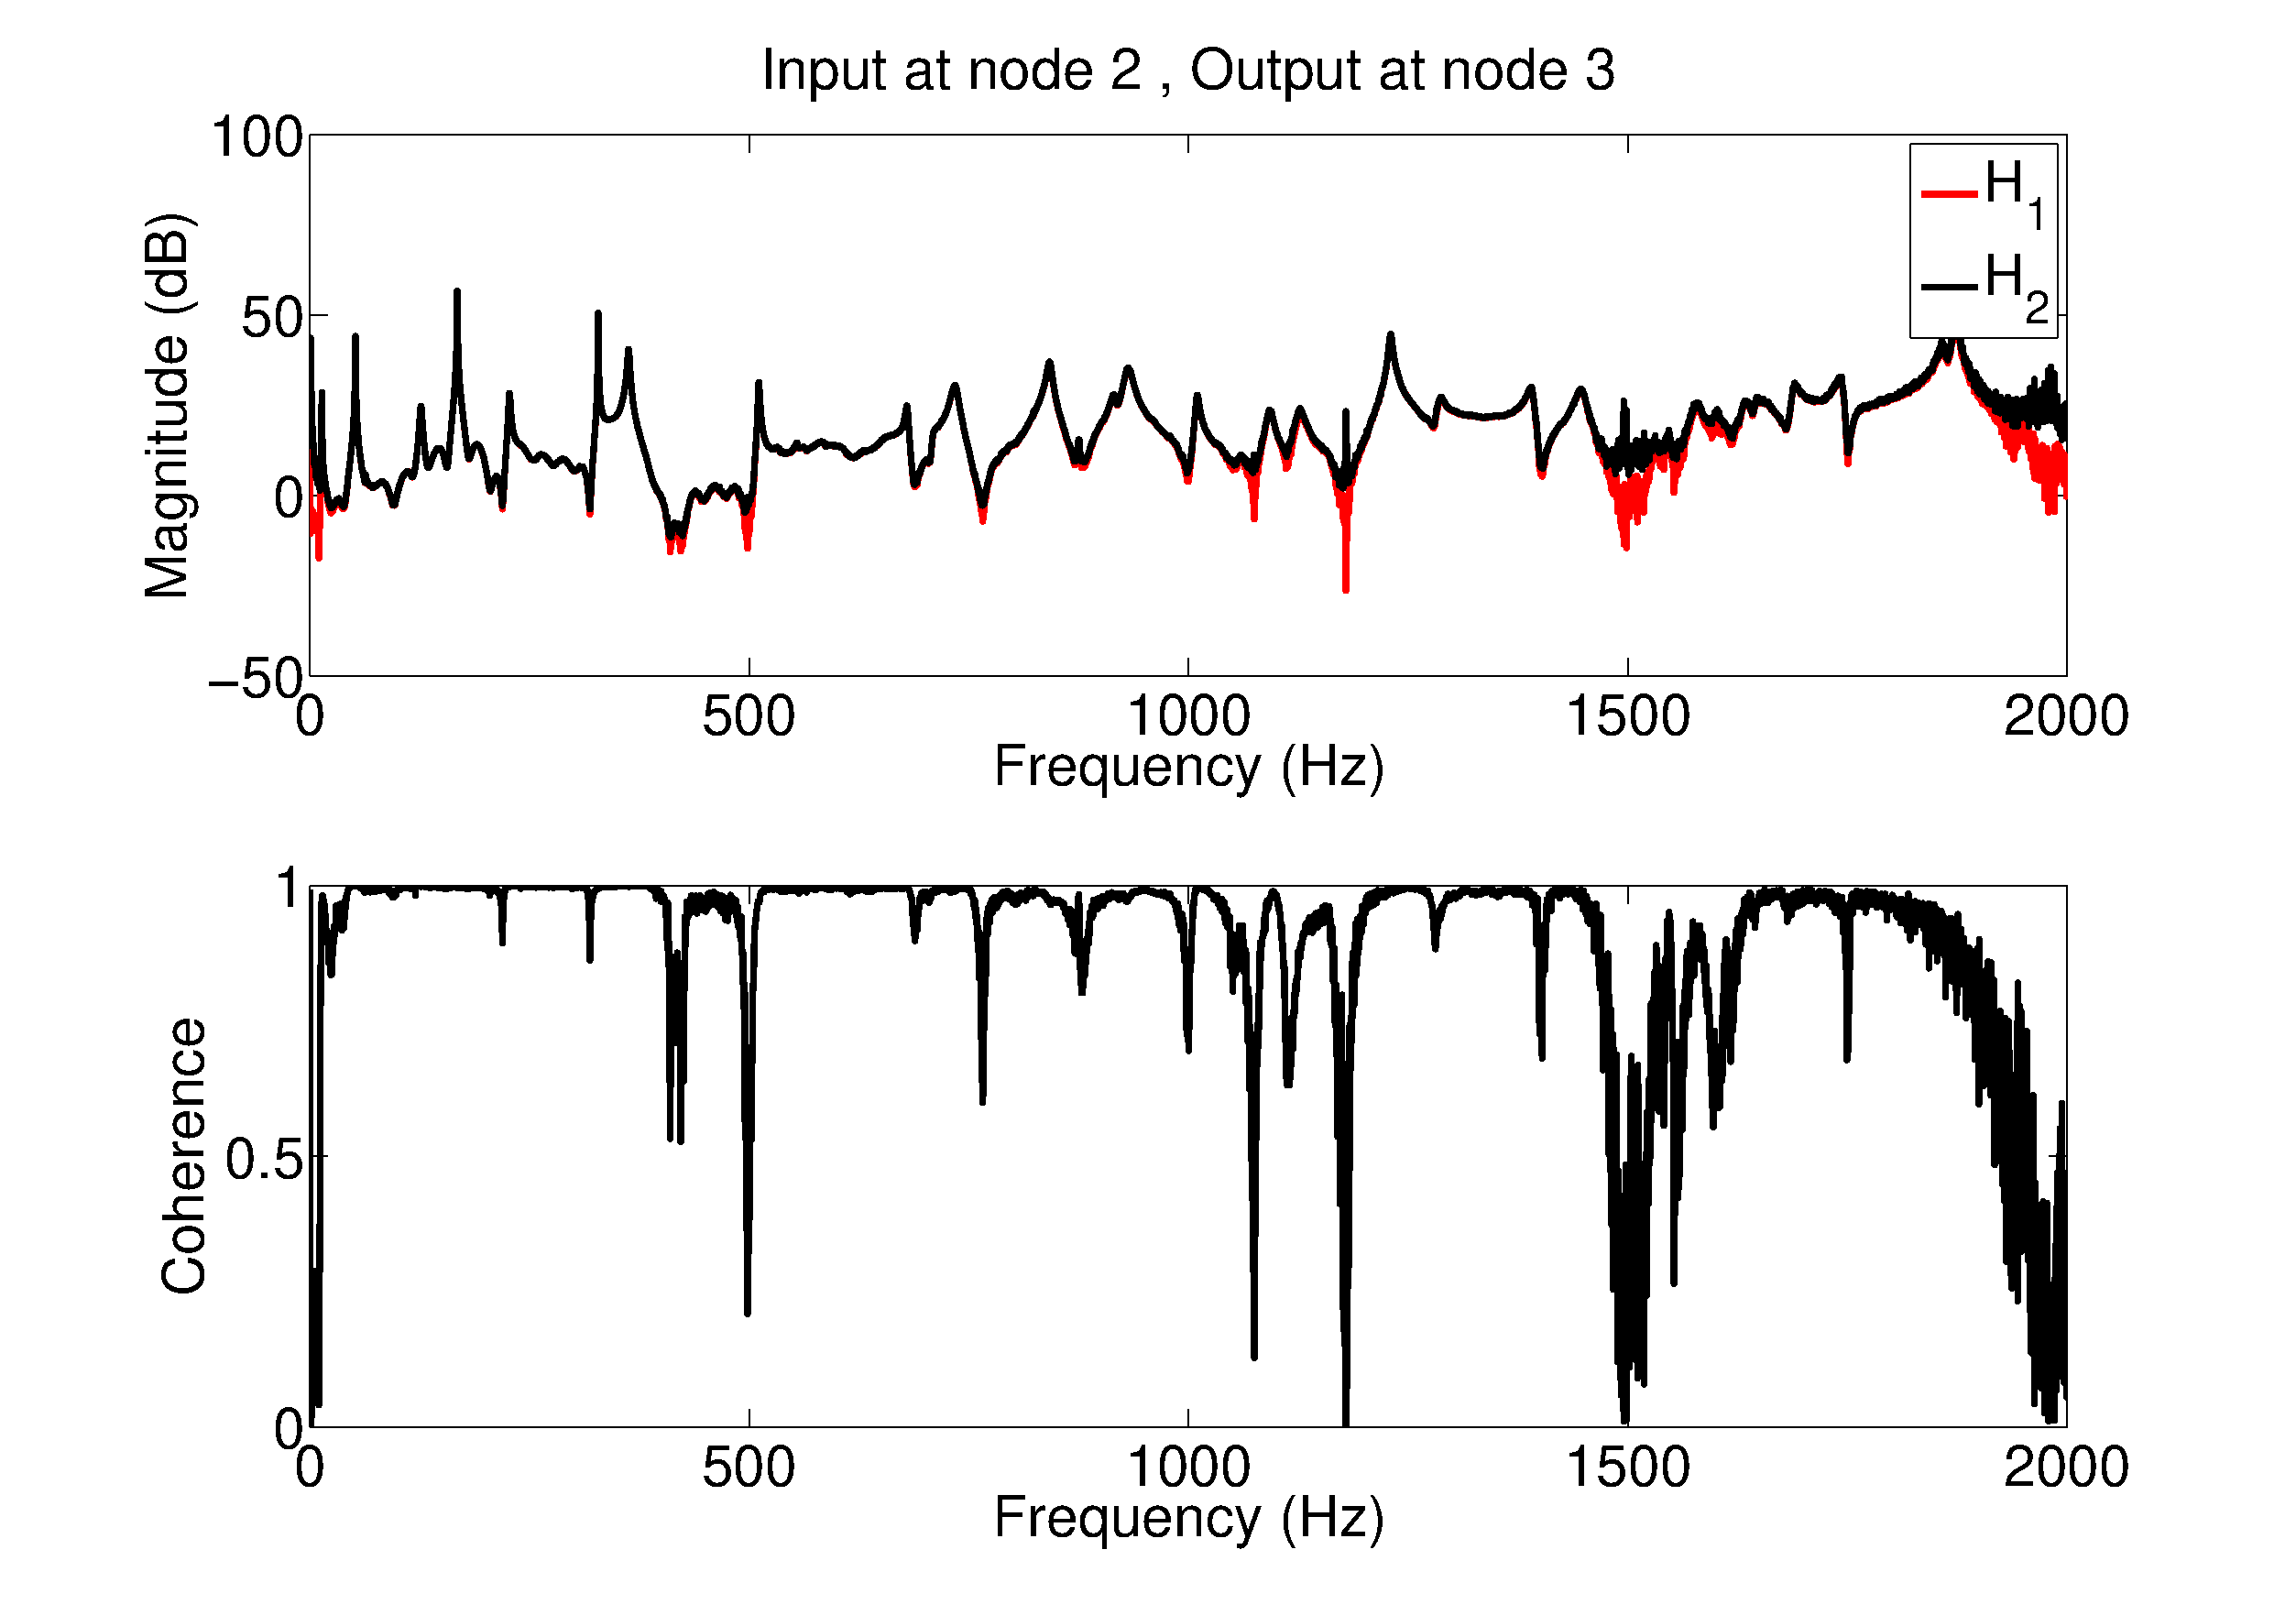
\includegraphics[height=4.75cm]{H32.eps}
	}
	\caption{Frequency response function for input at node 2.}
	\label{fig:all_FRFs_2}
\end{figure}
%
%
\begin{figure}[H]
	\centering
	\subfigure[]
	{
		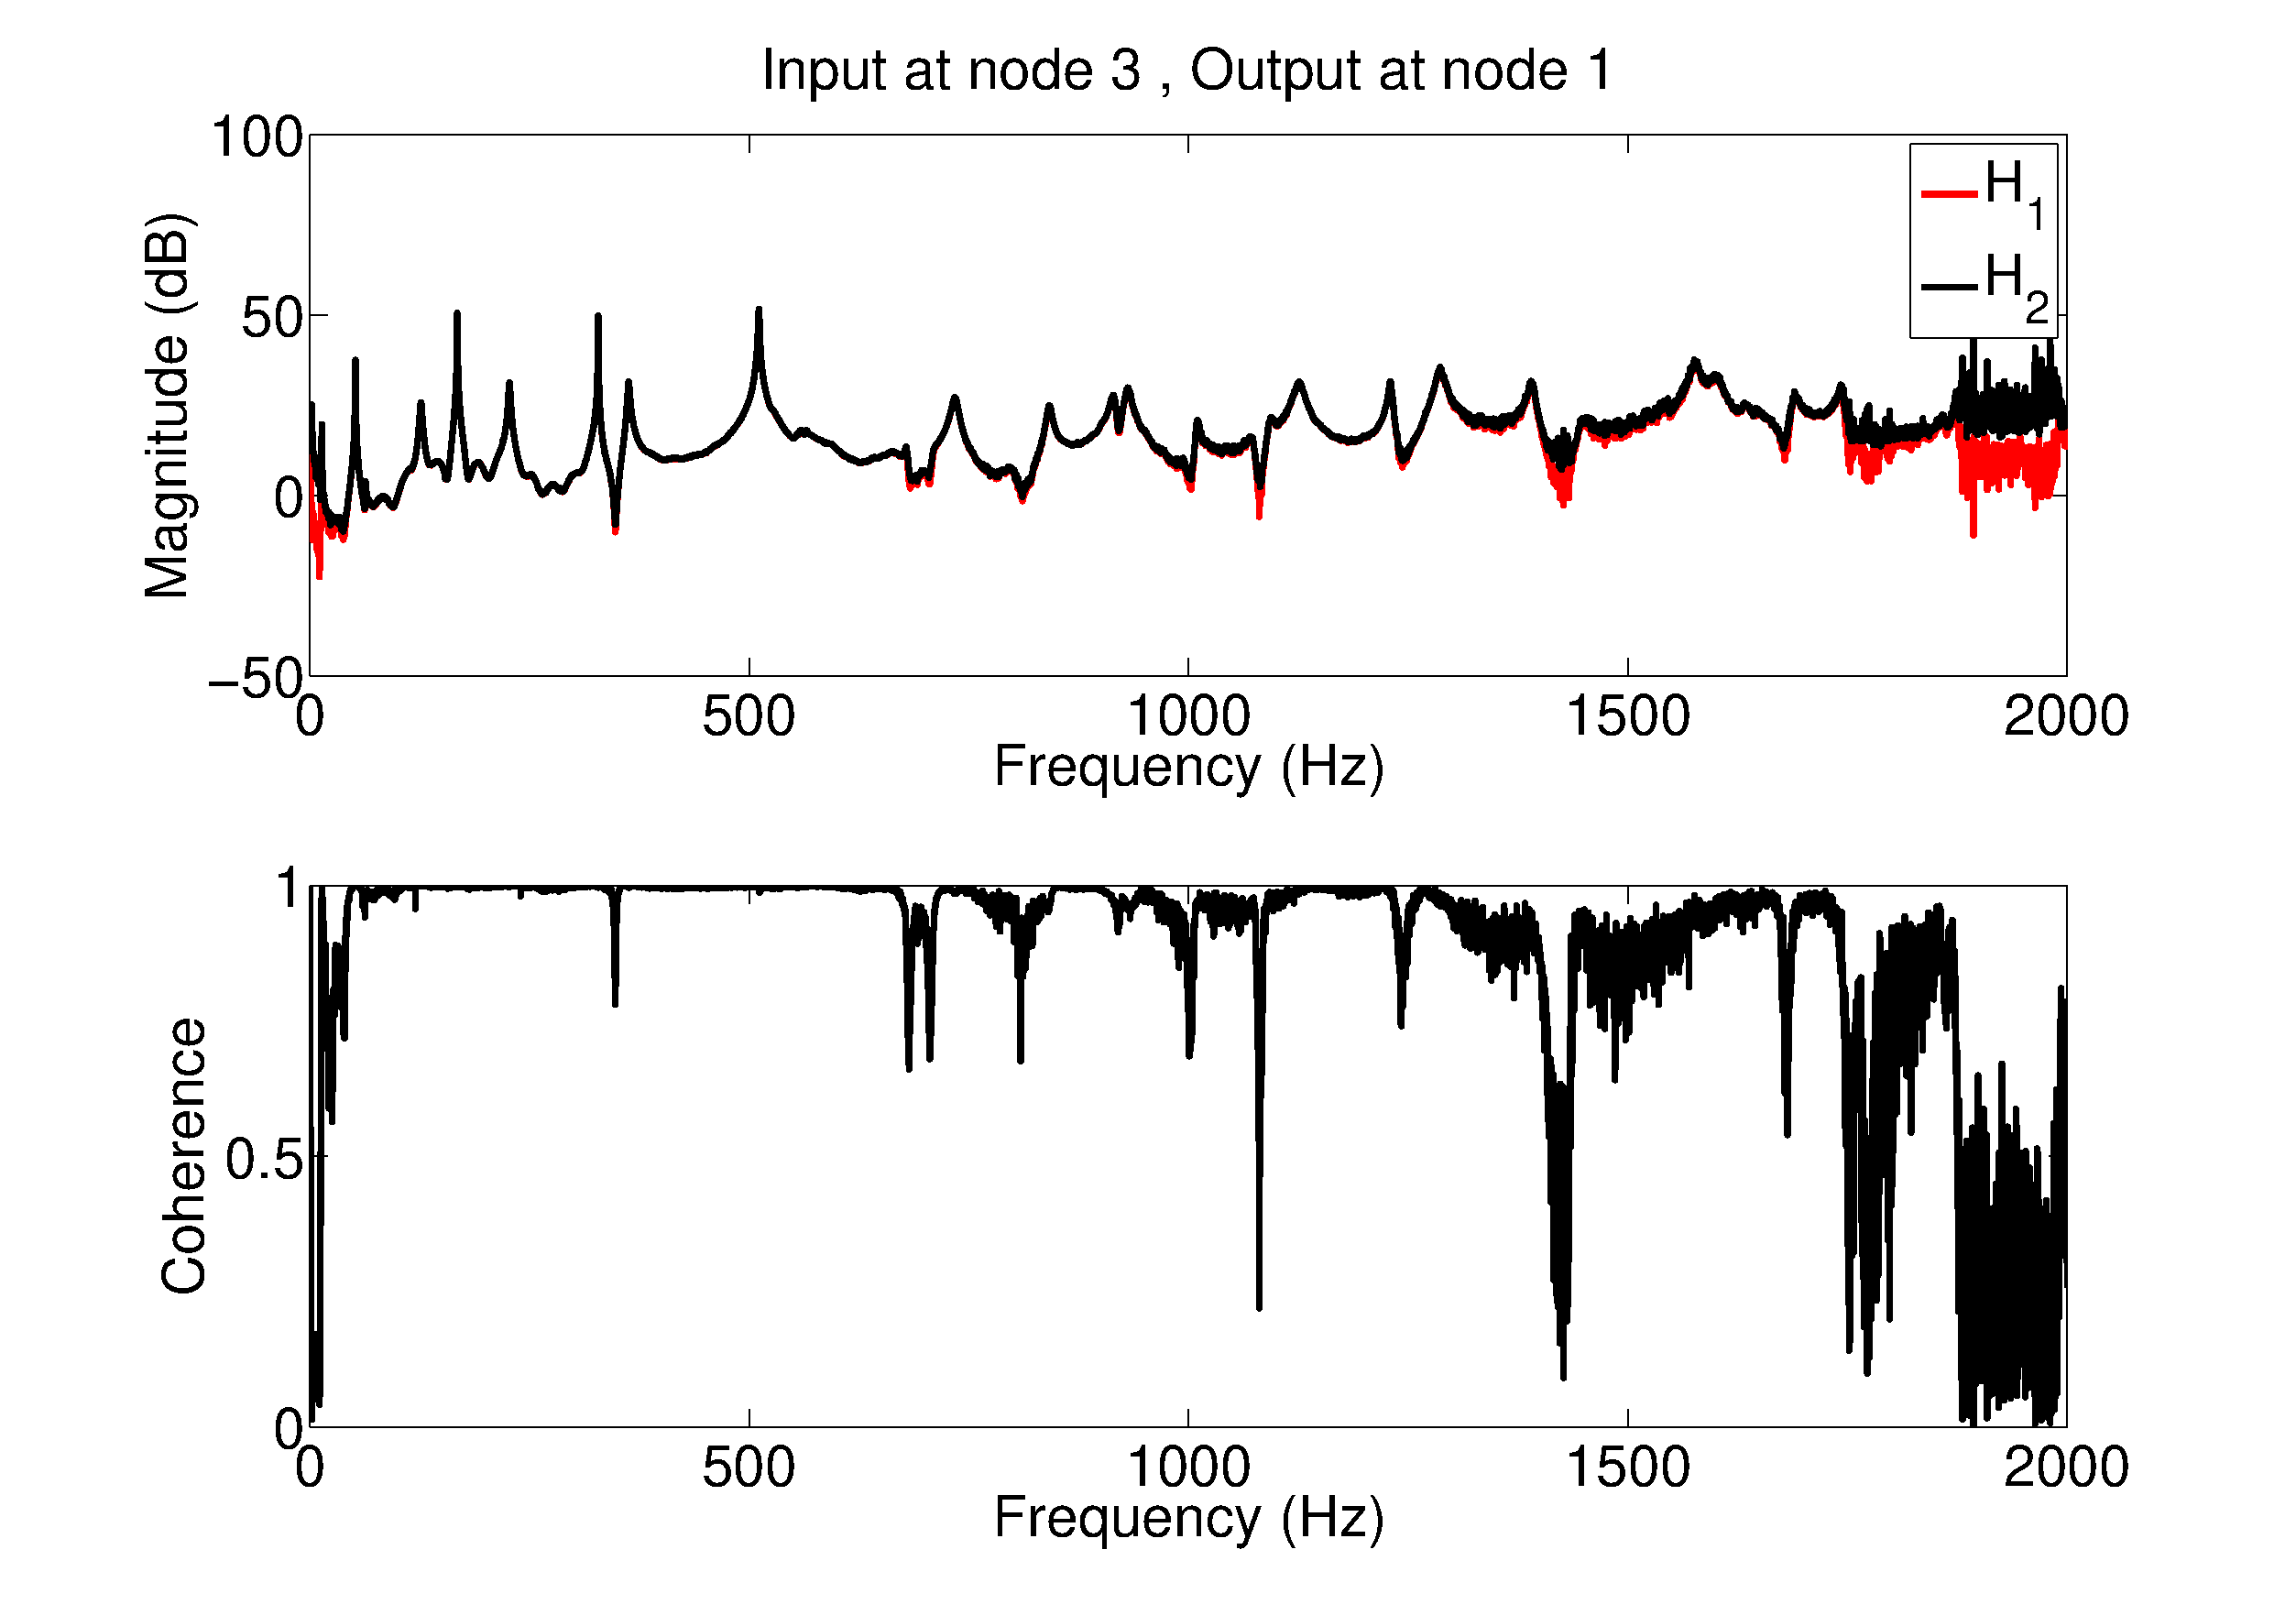
\includegraphics[height=4.75cm]{H13.eps}
	}
	\quad
	\subfigure[]
	{
		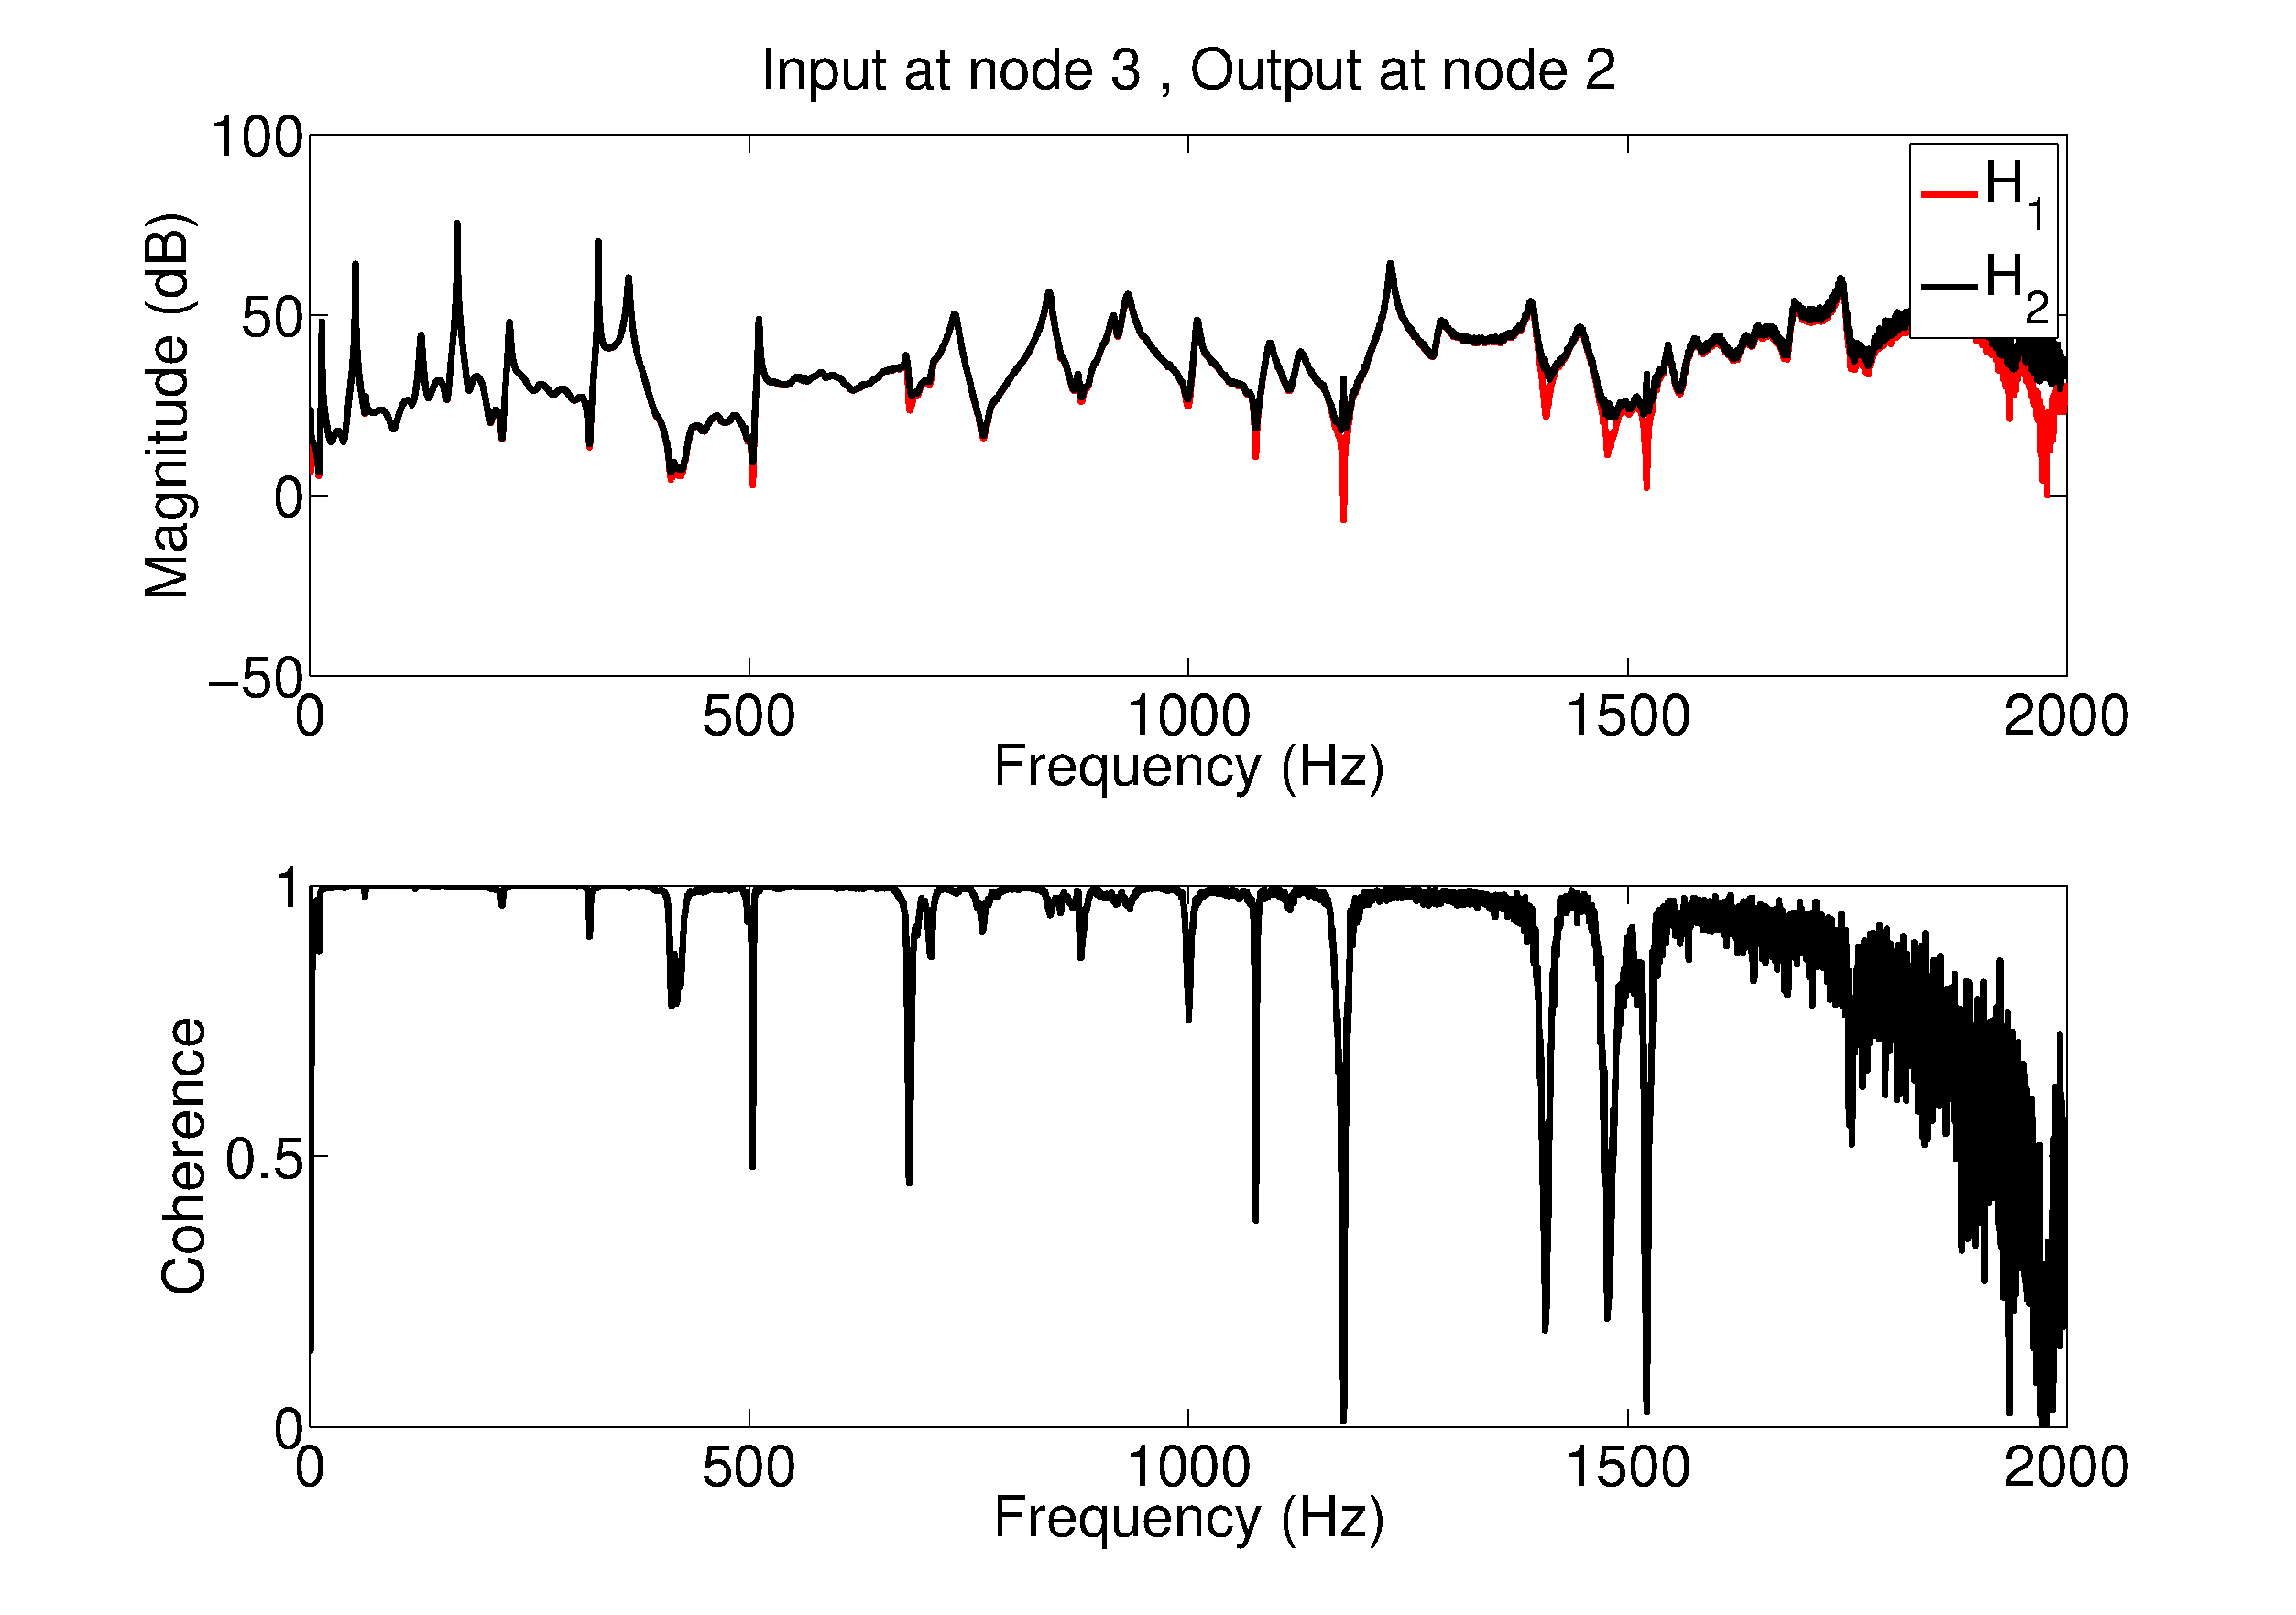
\includegraphics[height=4.75cm]{H23.eps}
	}
	\\
	\subfigure[]
	{
		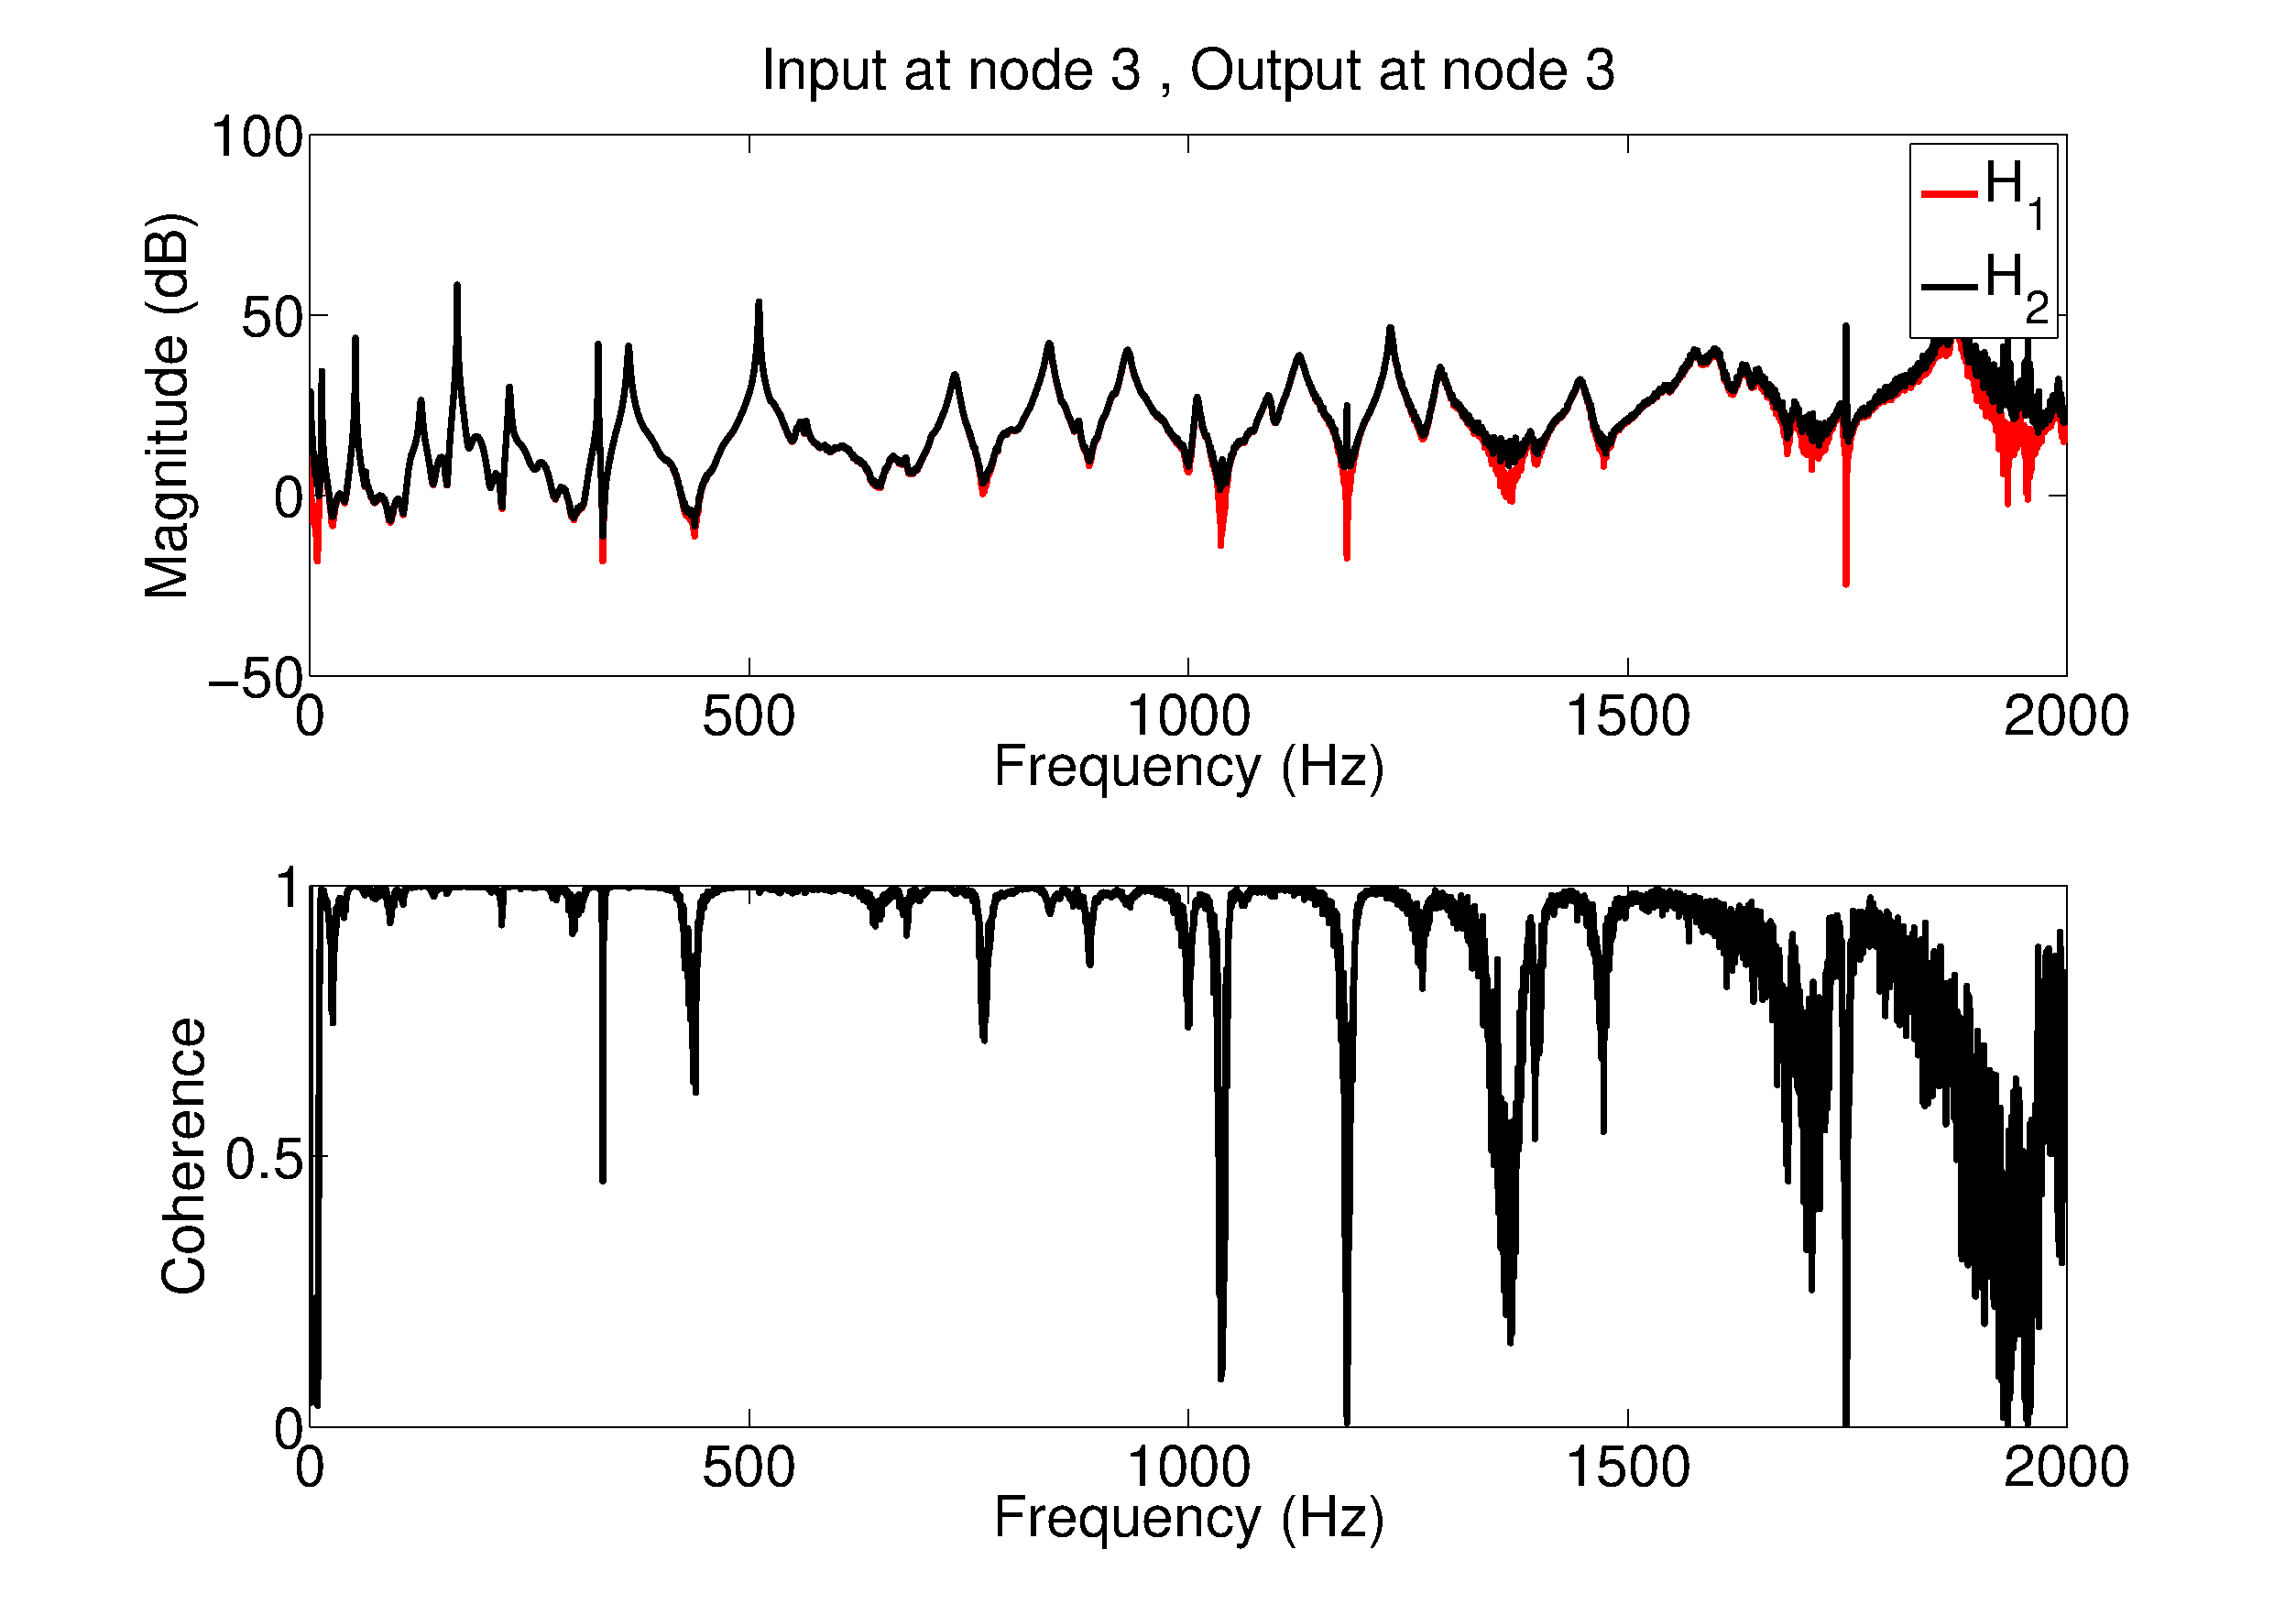
\includegraphics[height=4.75cm]{H33.eps}
	}
	\caption{Frequency response function for input at node 3.}
	\label{fig:all_FRFs_3}
\end{figure}
%
For the MDOF identification technique, we chose the frequency range of 220 Hz to 380 Hz. In this range, the coherence is near one for all the FRFs and also we can see three modes in the FRF data. This is required for the MDOF identification technique since we have three FRFs. The magnitude and phase of the FRFs for the specified frequency range is shown in Figure ~\ref{fig:range_FRF_1}, ~\ref{fig:range_FRF_2} and ~\ref{fig:range_FRF_3}. To use Equation \eqref{eq:MDOF}, the negative frequency range is also added to the frequency data. The FRF value in the negative frequency range is the complex-conjugate of the the FRF data. The system properties are calculated as follows.
%
\begin{gather*}
M = 
\begin{bmatrix}
	0.0064506 & 0.014113 & 0.02188 \\
	0.00043015 & 0.00084479 & 0.0013725 \\
	0.005462 & 0.013586 & 0.01835
\end{bmatrix}
\end{gather*}
%
%
\begin{gather*}
C = 
\begin{bmatrix}
	0.0026488 & 0.01265 & 0.0079285 \\
	0.032937 & 0.15733 & 0.098673 \\
	0.00079274 & 0.0037837 & 0.0023673
\end{bmatrix}
\end{gather*}
%
%
\begin{gather*}
K = 
\begin{bmatrix}
	1.49E-09 & 1.41E-08 & 2.20E-08 \\
	1.94E-08 & 1.14E-07 & 1.13E-07 \\
	2.00E-09 & 1.49E-08 & 2.03E-08
\end{bmatrix}
\end{gather*}
%
The matrices should have larger values. The low values of system properties are most probably due to having more than three modes in the sampled domain.
%
\begin{figure}[H]
	\centering
	\subfigure[]
	{
		\includegraphics[height=4.75cm]{H11_range.eps}
	}
	\quad
	\subfigure[]
	{
		\includegraphics[height=4.75cm]{H21_range.eps}
	}
	\\
	\subfigure[]
	{
		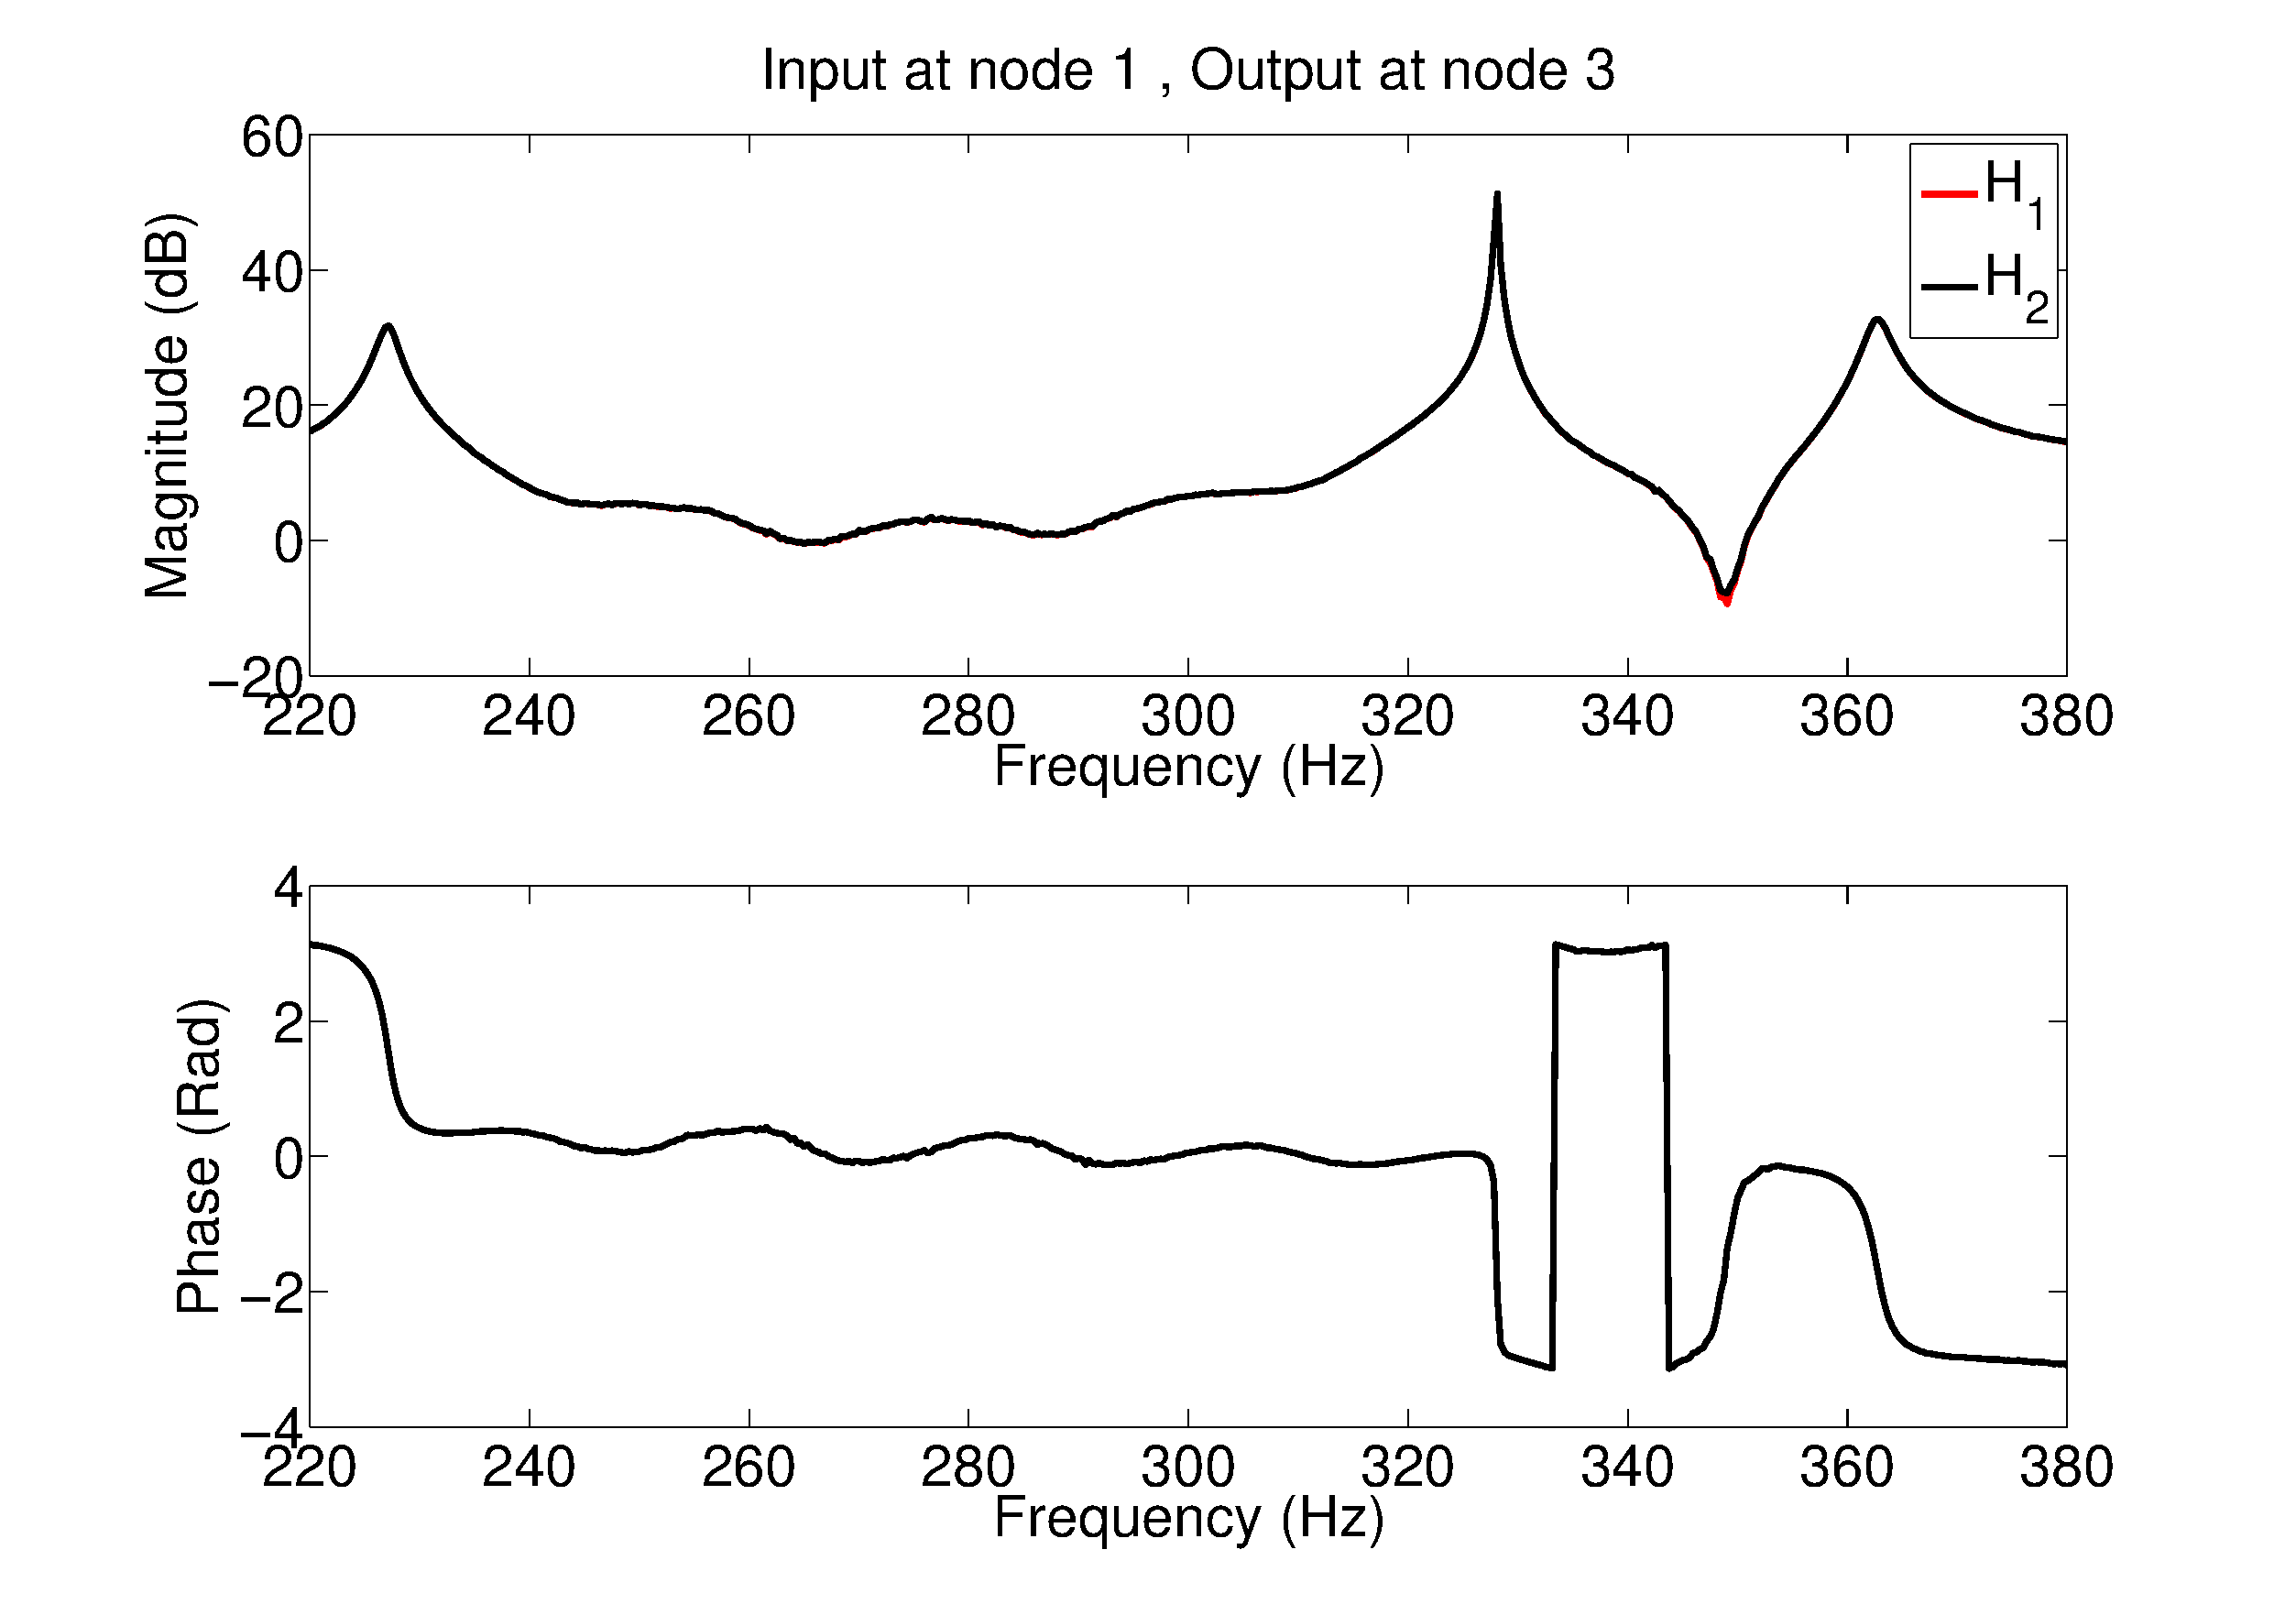
\includegraphics[height=4.75cm]{H31_range.eps}
	}
	\caption{Frequency response function for input at node 1.}
	\label{fig:all_FRFs_1}
\end{figure}
%
%
\begin{figure}[H]
	\centering
	\subfigure[]
	{
		\includegraphics[height=4.75cm]{H12_range.eps}
	}
	\quad
	\subfigure[]
	{
		\includegraphics[height=4.75cm]{H22_range.eps}
	}
	\\
	\subfigure[]
	{
		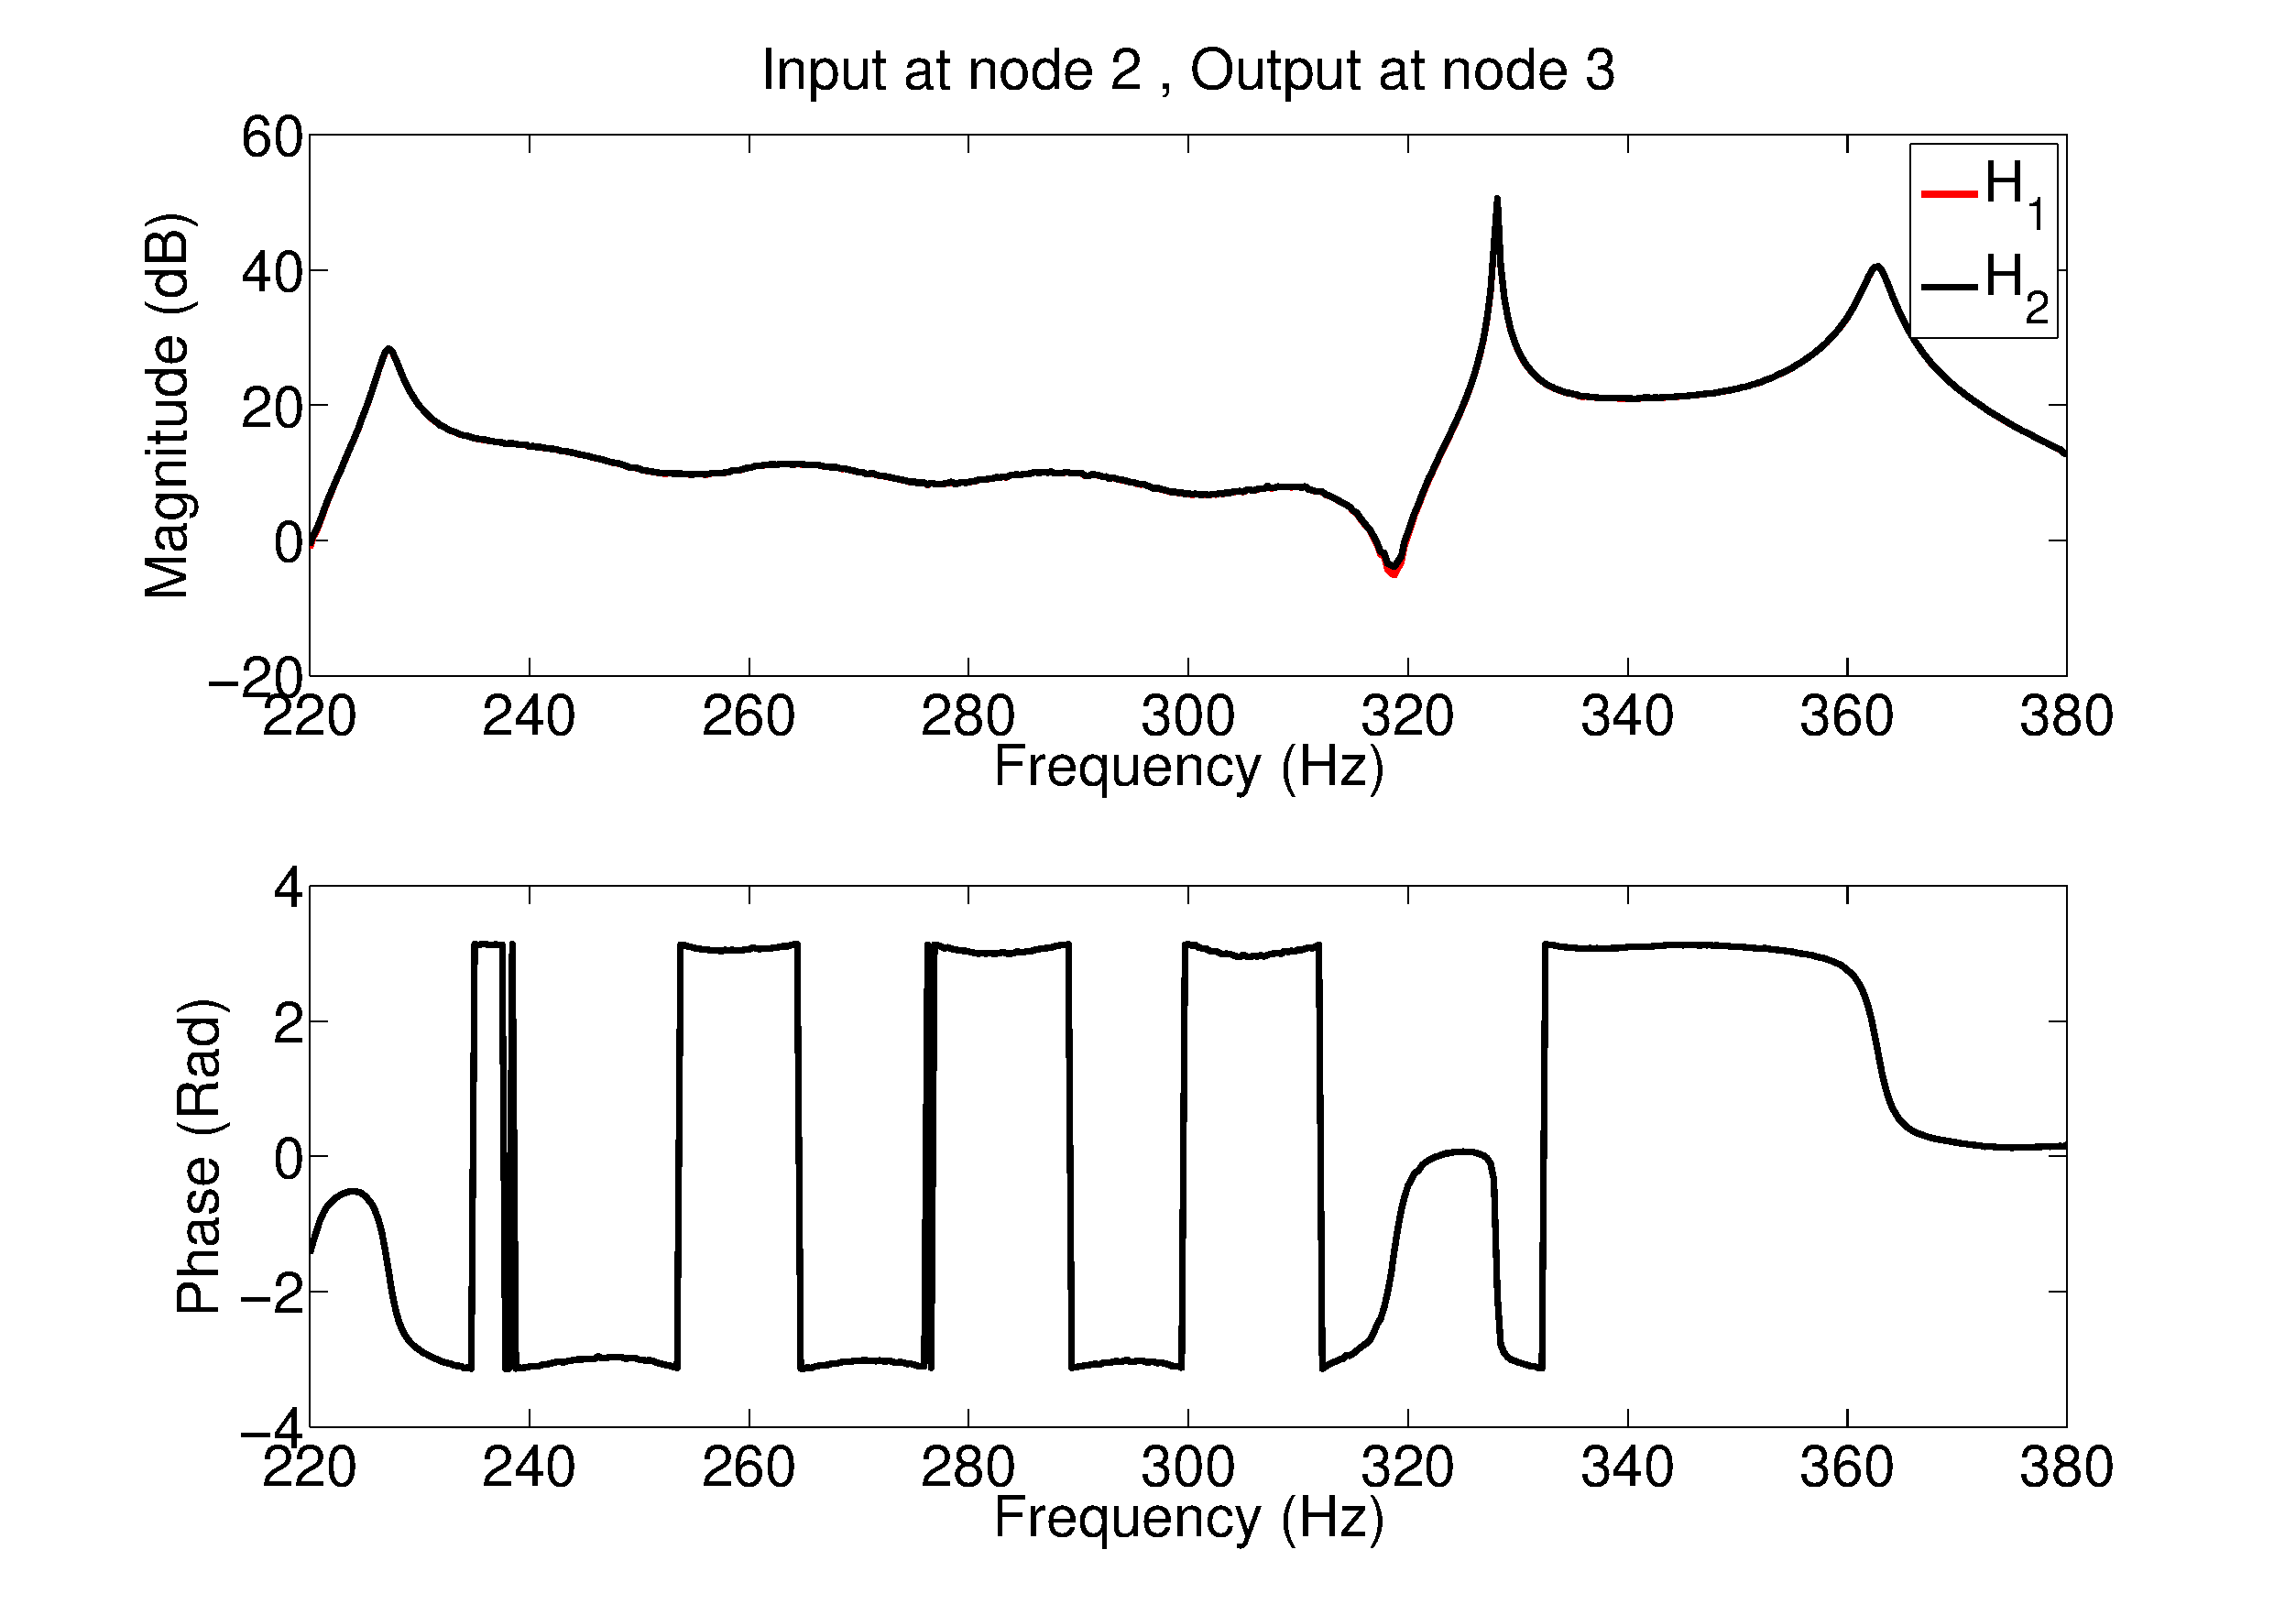
\includegraphics[height=4.75cm]{H32_range.eps}
	}
	\caption{Frequency response function for input at node 2.}
	\label{fig:all_FRFs_2}
\end{figure}
%
%
\begin{figure}[H]
	\centering
	\subfigure[]
	{
		\includegraphics[height=4.75cm]{H13_range.eps}
	}
	\quad
	\subfigure[]
	{
		\includegraphics[height=4.75cm]{H23_range.eps}
	}
	\\
	\subfigure[]
	{
		\includegraphics[height=4.75cm]{H33_range.eps}
	}
	\caption{Frequency response function for input at node 3.}
	\label{fig:all_FRFs_3}
\end{figure}
%
We have also used \lq\lq Single Degree of Freedom Curve Fitting with Residual\rq\rq\ to fit a curve to one of the peaks to calculate the natural frequency and the damping coefficient related to that peak. We chose $H_{31}$ as the FRF with the frequency range of 485 Hz to 540 Hz. This frequency isolates a peak as shown in Figure ~\ref{fig:SDOFwR}.
%
\begin{figure}[H]
	\centering
	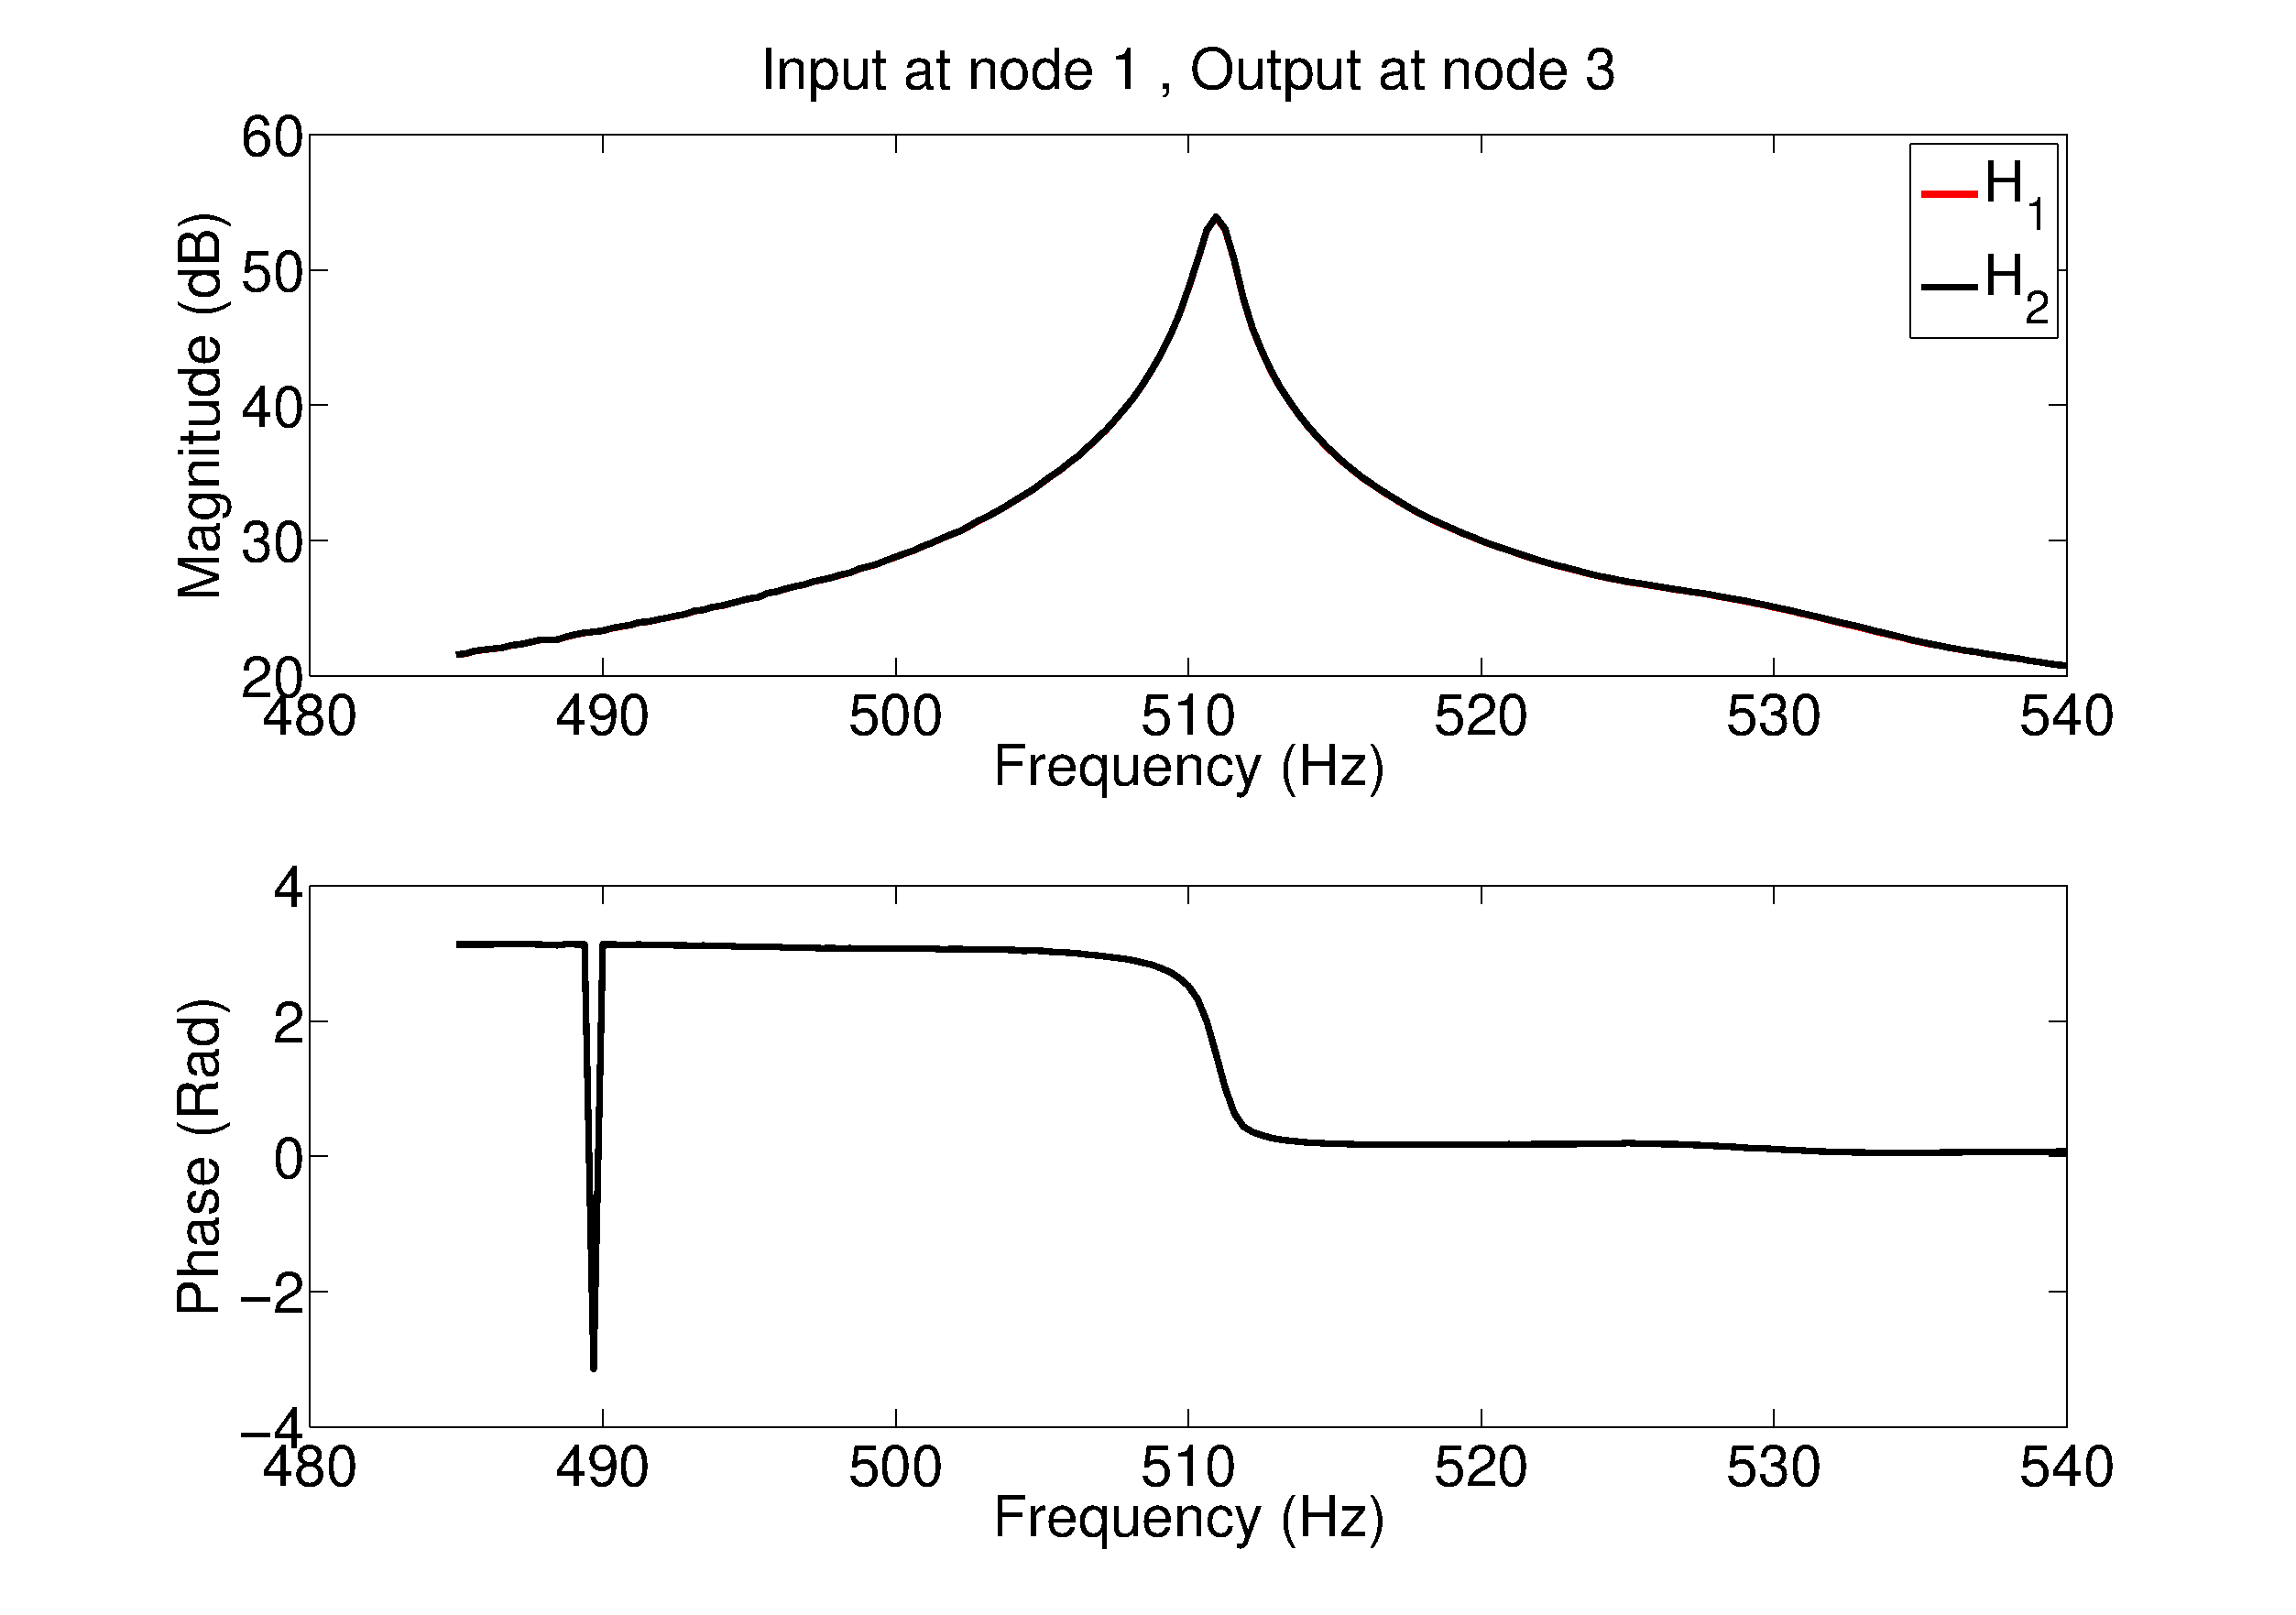
\includegraphics[height = 4.75cm]{H31_SDOF.eps}
	\caption{$H_{31}$ for SDOF curve fitting with residual method.}
	\label{fig:SDOFwR}
\end{figure}
%
In this method we have also added the negative frequency range to the frequency domain data. The FRF value for the negative frequency range is equal to the complex conjugate value of the FRF in the positive range. Using the experimental data and Equation \eqref{SDOFwR_matix} the natural frequency and damping coefficient is calculate as $510.81$ Hz and $0.00126$. The natural frequency agrees with what can be seen from the plot. The residue matrix is also shown in the following equation. Large values of this matrix indicate that the curve fit is not accurate.
%
\begin{gather}
\begin{bmatrix}
	\frac{1}{m_r} \\
	\frac{1}{k_r} \\
	b \\
	\bar{b}
\end{bmatrix}
=
\begin{bmatrix}
     0.21711 - 171.86i \\
     0.85579 + 8.1014e-05i \\
     -15.976 + 303.17i \\
     -15.992 + 303.17i
\end{bmatrix}
\end{gather}
%
%----------------------------------------------------------------------------------------
%	END
%----------------------------------------------------------------------------------------
\newpage
\section*{Appendix}
\subsection*{Extract Data From Bobcat Output}
\begin{lstlisting}
for inputLocation = 1:3
    Gfx_n1 = 0;
    Gxf_n1 = 0;
    Gff_n1 = 0;
    Gxx_n1 = 0;

    Gfx_n2 = 0;
    Gxf_n2 = 0;
    Gff_n2 = 0;
    Gxx_n2 = 0;

    Gfx_n3 = 0;
    Gxf_n3 = 0;
    Gff_n3 = 0;
    Gxx_n3 = 0;
    fileName = 'C:\Users\ecsroot\Desktop\Koorosh\Courses\ME7690_Vibration_testing
    	\Lab4\Data\';
    fileName = [fileName num2str(inputLocation)];
    for ii=1:10
        readName = [fileName '\' num2str(ii) '.mat'];
        load(readName)
        dt = Time_domain(2) - Time_domain(1);
        T = Time_domain(end);
        fs = 1 / dt;
        fNyq = 0.25 * fs;
        df = 1 / T;

        omega = Freq_domain;
        F = fft(Time_chan_1) * dt; F = F(1:length(omega));
        X1 = fft(Time_chan_2) * dt; X1 = X1(1:length(omega));
        X2 = fft(Time_chan_3) * dt; X2 = X2(1:length(omega));
        X3 = fft(Time_chan_4) * dt; X3 = X3(1:length(omega));

        % 'n' represents the input location. For 'far' it is (3) 
        Gfx_n1 = Gfx_n1 + conj(F) .* X1 / T;
        Gxf_n1 = Gxf_n1 + conj(X1) .* F / T;
        Gff_n1 = Gff_n1 + real(conj(F) .* F) / T;
        Gxx_n1 = Gxx_n1 + real(conj(X1) .* X1) / T;

        Gfx_n2 = Gfx_n2 + conj(F) .* X2 / T;
        Gxf_n2 = Gxf_n2 + conj(X2) .* F / T;
        Gff_n2 = Gff_n2 + real(conj(F) .* F) / T;
        Gxx_n2 = Gxx_n2 + real(conj(X2) .* X2) / T;

        Gfx_n3 = Gfx_n3 + conj(F) .* X3 / T;
        Gxf_n3 = Gxf_n3 + conj(X3) .* F / T;
        Gff_n3 = Gff_n3 + real(conj(F) .* F) / T;
        Gxx_n3 = Gxx_n3 + real(conj(X3) .* X3) / T;
    end
    Gfx_n1 = Gfx_n1 / 10;
    Gxf_n1 = Gxf_n1 / 10;
    Gff_n1 = Gff_n1 / 10;
    Gxx_n1 = Gxx_n1 / 10;

    Gfx_n2 = Gfx_n2 / 10;
    Gxf_n2 = Gxf_n2 / 10;
    Gff_n2 = Gff_n2 / 10;
    Gxx_n2 = Gxx_n2 / 10;

    Gfx_n3 = Gfx_n3 / 10;
    Gxf_n3 = Gxf_n3 / 10;
    Gff_n3 = Gff_n3 / 10;
    Gxx_n3 = Gxx_n3 / 10;

    H1_n1 = Gfx_n1 ./ Gff_n1;
    H2_n1 = Gxx_n1 ./ Gxf_n1;
    gamma_n1 = real(H1_n1 ./ H2_n1);

    H1_n2 = Gfx_n2 ./ Gff_n2;
    H2_n2 = Gxx_n2 ./ Gxf_n2;
    gamma_n2 = real(H1_n2 ./ H2_n2);

    H1_n3 = Gfx_n3 ./ Gff_n3;
    H2_n3 = Gxx_n3 ./ Gxf_n3;
    gamma_n3 = real(H1_n3 ./ H2_n3);

    nameH1_n1 = genvarname(['H1_1' num2str(inputLocation)]);
    assignin('base',nameH1_n1,H1_n1);
    namegamma_n1 = genvarname(['gamma_1' num2str(inputLocation)]);
    assignin('base',namegamma_n1,gamma_n1);
    nameH1_n2 = genvarname(['H1_2' num2str(inputLocation)]);
    assignin('base',nameH1_n2,H1_n2);
    namegamma_n2 = genvarname(['gamma_2' num2str(inputLocation)]);
    assignin('base',namegamma_n2,gamma_n2);
    nameH1_n3 = genvarname(['H1_3' num2str(inputLocation)]);
    assignin('base',nameH1_n3,H1_n3);
    namegamma_n3 = genvarname(['gamma_3' num2str(inputLocation)]);
    assignin('base',namegamma_n3,gamma_n3);

    clearvars -except H1_12 gamma_12 H1_22 gamma_22 H1_32 gamma_32 ...
                        H1_11 gamma_11 H1_21 gamma_21 H1_31 gamma_31 ...
                        H1_13 gamma_13 H1_23 gamma_23 H1_33 gamma_33 ...
                        inputLocation fontSize lineWidth omega
end
% close all;
H(1,1,:) = H1_11;
H(1,2,:) = H1_12;
H(1,3,:) = H1_13;
H(2,1,:) = H1_21;
H(2,2,:) = H1_22;
H(2,3,:) = H1_23;
H(3,1,:) = H1_31;
H(3,2,:) = H1_32;
H(3,3,:) = H1_33;

save 'H1_11.mat' H1_11
save 'H1_12.mat' H1_12
save 'H1_13.mat' H1_13
save 'H1_21.mat' H1_21
save 'H1_22.mat' H1_22
save 'H1_23.mat' H1_23
save 'H1_31.mat' H1_31
save 'H1_32.mat' H1_32
save 'H1_33.mat' H1_33
save 'H.mat' H
save 'omega.mat' omega
\end{lstlisting}
\subsection*{MDOF Curve Fitting}
\begin{lstlisting}
clc;
format short g;
close all;
fclose all;
clear all;
% ----------------------------------------------------------------------- %
lineWidth = 3;
fontSize = 20;
% ----------------------------------------------------------------------- %
load('C:\Users\ecsroot\Desktop\Koorosh\Courses\ME7690_Vibration_testing
	\Lab4\Matlab\H data\H1_13.mat')
load('C:\Users\ecsroot\Desktop\Koorosh\Courses\ME7690_Vibration_testing
	\Lab4\Matlab\H data\H1_21.mat')
load('C:\Users\ecsroot\Desktop\Koorosh\Courses\ME7690_Vibration_testing
	\Lab4\Matlab\H data\H1_22.mat')
load('C:\Users\ecsroot\Desktop\Koorosh\Courses\ME7690_Vibration_testing
	\Lab4\Matlab\H data\H1_23.mat')
load('C:\Users\ecsroot\Desktop\Koorosh\Courses\ME7690_Vibration_testing
	\Lab4\Matlab\H data\H1_31.mat')
load('C:\Users\ecsroot\Desktop\Koorosh\Courses\ME7690_Vibration_testing
	\Lab4\Matlab\H data\H1_32.mat')
load('C:\Users\ecsroot\Desktop\Koorosh\Courses\ME7690_Vibration_testing
	\Lab4\Matlab\H data\H1_33.mat')
load('C:\Users\ecsroot\Desktop\Koorosh\Courses\ME7690_Vibration_testing
	\Lab4\Matlab\H data\omega.mat')
load('C:\Users\ecsroot\Desktop\Koorosh\Courses\ME7690_Vibration_testing
	\Lab4\Matlab\H data\H.mat')
load('C:\Users\ecsroot\Desktop\Koorosh\Courses\ME7690_Vibration_testing
	\Lab4\Matlab\H data\H1_11.mat')
load('C:\Users\ecsroot\Desktop\Koorosh\Courses\ME7690_Vibration_testing
	\Lab4\Matlab\H data\H1_12.mat')

Hbig = [];
BtildeBig = [];
rangeMin = 220;
rangeMax = 380;
[r cMin] = min(abs(omega - rangeMin));
[r cMax] = min(abs(omega - rangeMax));

omega = omega * 2 * pi;
omegaR = omega(cMin:cMax);
omegaR = [fliplr(-omegaR')';omegaR];
HH = H(:,:,cMin:cMax);
H_ = zeros(3,3,length(omegaR));
for ii=1:length(omegaR)
    if omegaR(ii) < 0
        H_(:,:,ii) = conj(HH(:,:,length(HH) - ii + 1));
    else
        H_(:,:,ii) = HH(:,:,ii - length(HH));
    end
end

for ii=1:length(omegaR)
	Hbig = [Hbig;...
        -omegaR(ii)^2*H_(:,:,ii).' ...
        i*omegaR(ii)*H_(:,:,ii).' ...
        H_(:,:,ii).'];
    BtildeBig = [BtildeBig;eye(3,3) * -omegaR(ii)^2];
end

MCK = pinv(Hbig) * BtildeBig;

M = abs(MCK(1:3,1:3));
C = abs(MCK(4:6,1:3));
K = abs(MCK(7:9,1:3));
\end{lstlisting}
\subsection*{Single Degree of Freedom Curve Fitting with Residual}
\begin{lstlisting}
clc;
clear all;
format short g;
close all;
% ----------------------------------------------------------------------- %
load('C:\Users\ecsroot\Desktop\Koorosh\Courses\ME7690_Vibration_testing
	\Lab4\Matlab\H data\H1_13.mat')
load('C:\Users\ecsroot\Desktop\Koorosh\Courses\ME7690_Vibration_testing
	\Lab4\Matlab\H data\H1_21.mat')
load('C:\Users\ecsroot\Desktop\Koorosh\Courses\ME7690_Vibration_testing
	\Lab4\Matlab\H data\H1_22.mat')
load('C:\Users\ecsroot\Desktop\Koorosh\Courses\ME7690_Vibration_testing
	\Lab4\Matlab\H data\H1_23.mat')
load('C:\Users\ecsroot\Desktop\Koorosh\Courses\ME7690_Vibration_testing
	\Lab4\Matlab\H data\H1_31.mat')
load('C:\Users\ecsroot\Desktop\Koorosh\Courses\ME7690_Vibration_testing
	\Lab4\Matlab\H data\H1_32.mat')
load('C:\Users\ecsroot\Desktop\Koorosh\Courses\ME7690_Vibration_testing
	\Lab4\Matlab\H data\H1_33.mat')
load('C:\Users\ecsroot\Desktop\Koorosh\Courses\ME7690_Vibration_testing
	\Lab4\Matlab\H data\omega.mat')
load('C:\Users\ecsroot\Desktop\Koorosh\Courses\ME7690_Vibration_testing
	\Lab4\Matlab\H data\H.mat')
load('C:\Users\ecsroot\Desktop\Koorosh\Courses\ME7690_Vibration_testing
	\Lab4\Matlab\H data\H1_11.mat')
load('C:\Users\ecsroot\Desktop\Koorosh\Courses\ME7690_Vibration_testing
	\Lab4\Matlab\H data\H1_12.mat')

rangeMin = 485;
rangeMax = 540;
[r cMin] = min(abs(omega - rangeMin));
[r cMax] = min(abs(omega - rangeMax));
omegaR = omega(cMin:cMax);
omegaR = [fliplr(-omegaR')';omegaR];
H_31R = H1_31(cMin:cMax);
H_31R = [fliplr(conj(H_31R'))';H_31R];

P = [(i * omegaR).^2 .* H_31R, ...
    (i * omegaR).^3 .* H_31R, ...
    -(i * omegaR).^0, ...
    -(i * omegaR).^1, ...
    -(i * omegaR).^2, ...
    -(i * omegaR).^3, ...
    -(i * omegaR).^4];
BETA_ALPHA = pinv(P) * (-(i * omegaR).^4 .* H_31R);
BETA = fliplr([0 0 (BETA_ALPHA(1:2,1)).' 1]);
LAMBDA = roots(BETA);

OMEGA_n = abs(LAMBDA)
ZETA = - real(LAMBDA) ./ abs(LAMBDA)

pinv([-1./omegaR, ...
    ones(length(omegaR),1), ...
    1 ./ (i * omegaR - LAMBDA(3)), ...
    1 ./ (i * omegaR - LAMBDA(4))]) * H_31R;
\end{lstlisting}
%----------------------------------------------------------------------------------------
%	END
%----------------------------------------------------------------------------------------
\end{document}